% This is LLNCS.DEM the demonstration file of
% the LaTeX macro package from Springer-Verlag
% for Lecture Notes in Computer Science,
% version 2.4 for LaTeX2e as of 16. April 2010
%
\documentclass{llncs}
%\documentclass[runningheads]{llncs}

% *** GRAPHICS RELATED PACKAGES ***
\usepackage{graphicx}
% declare the path(s) where your graphic files are
\graphicspath{{./Figs/}}
% and their extensions so you won't have to specify these with
% every instance of \includegraphics
\DeclareGraphicsExtensions{.pdf,.jpeg,.png}

%% ------ Packages added by pete ------ %%
%% ------ packages for authors format  ------ %%
\usepackage[misc]{ifsym}
\usepackage{bbding}
\usepackage{url}

\urldef{\mailsa}\path|{yuwenping}@mail.nankai.edu.cn|
\urldef{\mailsb}\path|{zhangjz, xujd, xuyw}@nankai.edu.cn|
%% ------ packages for authors format  ------ %%

%% ------ packages for subfigures  ------ %%
\usepackage[caption=false,font=footnotesize]{subfig}
%\usepackage{caption}
%\usepackage[justification=centering]{caption}

%% ------ packages for algorithm expressed with the pseudocode  ------ %%
\usepackage{algorithm}
%\usepackage{algorithmic}
\usepackage{algcompatible}

%% ------ packages for list  ------ %%
%\usepackage{enumitem}% http://ctan.org/pkg/enumitem


%% ------ typesetting with little spacing ------ %%
%%% Save the class definition of \subparagraph
%\let\llncssubparagraph\subparagraph
%%% Provide a definition to \subparagraph to keep titlesec happy
%\let\subparagraph\paragraph
%%% Load titlesec
%\usepackage[compact]{titlesec}
%%% Revert \subparagraph to the llncs definition
%\let\subparagraph\llncssubparagraph

\begin{document}

%%
%\mainmatter              % start of the contributions
%
\title{AiFiMatch: Accurate Indoor Map Matching Algorithm Based on Activity Detection and Crowd-sourced Wi-Fi}
%J
\titlerunning{AiFiMatch}  % abbreviated title (for running head)
%                                     also used for the TOC unless
%                                     \toctitle is used
%
%%\author{Wenping Yu\inst{1}}

\author{Jianzhong Zhang$^2$ $^($\Envelope$^)$ \and Wenping Yu$^1$ \and Jingdong Xu$^2$ \and Yuwei Xu$^2$}
%
\authorrunning{Wenping Yu et al.} % abbreviated author list (for running head)
%
%%%% list of authors for the TOC (use if author list has to be modified)
\tocauthor{Wenping Yu}
%
\institute{College of Computer and Control Engineering, Nankai University, Tianjin, China\\
$^1$\mailsa\\
$^2$\mailsb\\}


\maketitle              % typeset the title of the contribution

\begin{abstract}

Map matching has been widely investigated in indoor pedestrian navigation to improve positioning accuracy and robustness. In this paper, we present AiFiMatch: a map matching algorithm that can provide accurate pedestrian walking trajectory tracking based on Hidden Markov Model (HMM). AiFiMatch abstracts the indoor map using a directed graph model in which the location-related activities, such as turning, walking stairs, are directed edges, and indoor road segments between these special locations are nodes. With the help of a novel HMM model, AiFiMatch maps pedestrian's walking trajectory subset sequence to indoor map based on activity detection (AD). Simultaneously, Wi-Fi fingerprints can be bound to physical locations by timestamp. AiFiMatch can automatically construct and update radio map of indoor road segments via crowdsourcing. With this radio map, AiFiMatch  efficiently solves the multiple hypotheses problem. We have evaluated our proposed algorithm using smartphones in the fifth floor of a teaching building on campus. Experimental results show that AiFiMatch can accurately track a pedestrian even without knowing the initial position and is robust to a certain degree of step length and heading direction estimation errors in the experimental environment. The mean offline positioning error is about $1.24$ m. The results also demonstrate that AiFiMatch significantly improves the convergence speed in buildings with Wi-Fi infrastructure.

%\keywords{Map Matching, Hidden Markov Model, Activity Detection, Crowdsourced Wi-Fi}
\keywords{Map Matching  \and Hidden Markov Model \and Activity Detection \and Crowdsourced Wi-Fi.}
\end{abstract}
%
\section{Introduction}
%
Location based services (LBS) have spilled over into all aspects of people's daily life. Outdoors, global positioning system (GPS) has been able to provide a reasonably good positioning \cite{zampella2015indoor}. However, robust and effective indoor pedestrian positioning is still at its infancy due to the blockage of GPS signals.

It is common for indoor positioning schemes to leverage pre-installed infrastructure like Wi-Fi\cite{bahl2000enhancements}, UWB\cite{Fontana2002}, RFID\cite{ni2004landmarc}, Bluetooth\cite{zafari2015enhancing}, and so on. These systems offer absolute positioning with a limited error level,but rely on expensive hardware or time-consuming pre-training. At present, motion sensors, including accelerometer, gyroscope and magnetometer, are widely used in smartphones. Therefore, dead reckoning (DR) technique using motion sensors is another way for indoor positioning, which derives the current position by adding the estimated displacement to the previous one. DR technique is known as pedestrian dead reckoning (PDR) for pedestrian tracking and positioning \cite{fu2017crowdsourcing,alaoui2017points,zhou2015activity}. The PDR technique itself does not provide a final solution to the pedestrian positioning problem and another technique is required to provide the initial position estimates.

The positioning error of PDR technique mainly comes from step length and direction estimation errors and even minor errors will be magnified by cumulation over time. Indoor map information may be connected with PDR, namely map matching algorithm \cite{aly2015semmatch}. Several map matching algorithms have been proposed to constrain the cumulative errors \cite{zhou2015activity,aly2015semmatch,zhou2015alimc,abdelnasser2016semanticslam,qiu2017iframe}.  One algorithm uses activity-related locations as virtual landmarks to find the optimal trajectory of a pedestrian. The activity-related locations are special points of a building, such as elevator, stair, corner, and so on. When a pedestrian passes these locations, the pedestrian's activities can be distinguished from normal walking. Human activity detection algorithms based on smartphones have attracted more and more researchers' attention in the past decade. Given the symmetry of indoor environment, activity-based map matching algorithms fails since there may be more than one alternatives for the same activity feature or activity sequence \cite{zhou2015activity}.

Crowdsourcing is a low-cost and efficient way to extract useful information from data acquired by crowd participants \cite{wang2016indoor}. The crowdsourcing method has been successfully applied to construct Wi-Fi fingerprint database \cite{zhang2014robust,xiang2017tack}. At present, Wi-Fi access points have been widely developed in public buildings. Meanwhile, almost all smartphones are equipped with Wi-Fi interfaces. Hence, It is feasible to introduce Wi-Fi signal feature, such as received signal strength (RSS), into map matching algorithms \cite{newson2009hidden,seitz2010hidden} to improve the positioning performance. Furthermore, Wi-Fi RSS can be used as a new feature to deal with the multiple hypotheses problem due to the symmetry of indoor environments.

We therefore propose AiFiMatch: a map matching algorithm based on a novel HMM model, which integrates activity-based map matching and crowdsourced Wi-Fi. During pedestrians walking, many smartphones can simultaneously collect motion sensors' data and Wi-Fi RSS values. On the one hand, AiFiMatch uses motion sensors' data to detect the pedestrian's location-related activities, divides the walking trajectory into sub-trajectory sequence and realizes pedestrian positioning based on PDR even without knowing the initial position by matching the sub-trajectory sequence to indoor road map. On the other hand, according to map matching results, WiFi RSS fingerprints can be bound to physical locations. As time goes by, a Wi-Fi fingerprint database can be built even further by crowdsourcing. This paper defines the dissimilarity between Wi-Fi RSS sequences. With the help of crowdsourced Wi-Fi fingerprint database, this dissimilarity can be used to reduce the number of candidate hidden states in the presented HMM model and even eliminate the symmetry of indoor environment. Thus, AiFiMatch can get the pedestrian's position estimations within a short time delay. 

%In summary, this paper's mainly contributions are as follows:
%\vspace{-10pt}
%\begin{itemize}
%	\setlength{\parskip}{0pt} 
%	\setlength{\itemsep}{0pt plus 1pt}
%	\renewcommand{\labelitemi}{$\vcenter{\hbox{\tiny$\bullet$}}$}
%	\item we present the architecture of AiFiMatch: a map matching algorithm based on activity detection and crowd-sourced Wi-Fi.
%	\item we present the architecture of AiFiMatch: a map matching algorithm based on activity detection and crowd-sourced Wi-Fi.
%\end{itemize}
%\vspace{-8pt}

%In summary, this paper's mainly contributions are as follows:
%\begin{itemize}[noitemsep,topsep=0pt]
%	\renewcommand{\labelitemi}{$\vcenter{\hbox{\tiny$\bullet$}}$}
%	\item we present the architecture of AiFiMatch: a map matching algorithm based on activity detection and crowd-sourced Wi-Fi.
%	\item we present the architecture of AiFiMatch: a map matching algorithm based on activity detection and crowd-sourced Wi-Fi.
%\end{itemize}

The remainder of this paper is organized as follows: Section II reviews the related work in the literature. Section III gives an overview of the AiFiMatch system and its preprocessing components. Then, we detail the proposed HMM-based map matching algorithm in Section IV. Section V shows the experimental results and analysis of the AiFiMatch system. Finally, Section VI concludes this paper.

\section{Related Work}

PDR techniques relying on smartphones have attracted much attention in the past few years, but we only position the literature with respect to our work in this section. We focus on techniques that utilize easily accessible infrastructure, such as indoor map information, inertial sensors embedded in smartphones and wireless access points in buildings. We divide these techniques into the following three categories: map information assisted PDR, activity detection based PDR and combination PDR with Wi-Fi Fingerprint. 

\subsection{Map Information Assisted PDR}

The pedestrian motion trajectory is restricted by the indoor map, therefore, it is an opportunity to improving PDR using map information. Woodman and Harle propose a pedestrian positioning approach which combines a detailed building map model and a particle filter to provide absolute positioning \cite{woodman2008pedestrian}. An improved particle filter is also introduced into map matching in \cite{bao2013indoor} and its computational complexity is less than traditional ones. Map matching algorithm is triggered only when a pedestrian is considered walking along a certain corridor. \cite{rai2012zee} leverages the topology of the indoor map to filter out infeasible locations over time with the particle filter. However, the computation time is still the major issues of particle filter based map matching algorithms, as a large number of particles are required to ensure good estimations. MapCraft proposed in \cite{xiao2014lightweight} expresses the map matching based pedestrian positioning problem as a conditional random field (CRF), which is extremely computationally efficient and tracks well even when presented with very noisy sensor data. Both MapCraft and our work only require a floor plan to track pedestrians, but a crowd-sourced Wi-Fi fingerprints database could be built by our work when wireless access points exist. 

\subsection{Activity Detection based PDR}

An activity detection based PDR system limits the cumulative errors by recognizing pedestrians' activities and matching their activities to corresponding locations. A random forest classifier is applied to classify consecutive activities relevant to positions in multi-floor buildings in \cite{bobkov2015activity}, such as walking, stairs up and stairs down. To prevent cumulation of PDR errors, inertial sensor features are used as virtual landmarks to match the special locations of positioning areas \cite{guo2017activity}. However, the ambiguity of the virtual landmark is not considered. In \cite{zhou2015activity}, a HMM model is used to match the activity sequence of smartphone user to the corresponding landmarks of indoor map. This approach can avoid the mismatch problem caused by the ambiguity of the virtual landmark. The hidden states and observations from the HMM model are different from the one presented in this work. We implement this approach and compare it with our work based on our own experimental data. SemanticSLAM proposed in \cite{abdelnasser2016semanticslam} discovers semantic landmarks in a crowd-sensing approach based on the data collected from the smartphone users. A semantic landmark is defined by two attributes: its sensors pattern and physical location. Each sensors pattern corresponds to one kind of activity of the smartphone users in buildings. ALIMC \cite{zhou2015alimc} uses the activity-related location as the landmark to merge the crowdsourcing trajectories. This approach can automatically construct indoor maps without any prior knowledge. All these SLAM approaches can be viewed as map generators providing digital indoor maps to our map matching algorithm.

\subsection{Combining PDR with Wi-Fi Fingerprint}

Wireless access points are widely developed these days in many buildings and Wi-Fi fingerprinting is a well-known localization technique. Combination PDR with Wi-Fi fingerprint tries to avoid the disadvantages of these two approaches. WiFi-SLAM \cite{Ferris2007WiFi} is a pioneer in fusing Wi-Fi RSS and motion sensor data. It simultaneously builds a map of the environment and locates the user within this map. A modified HMM model for the fusion of Wi-Fi fingerprinting and PDR is presented in \cite{hoang2013hidden}. For this approach, a pre-trained Wi-Fi fingerprint database is required. HiMLoc \cite{radu2013himloc} integrates PDR with indoor landmarks detection and Wi-Fi fingerprinting by a distributed particle filter. In spite of computational complexity, this approach, like our work, can provide continuous update of the training set of Wi-Fi fingerprints.

\section{AiFiMatch Overview}

AiFiMatch is an activity-based map matching system applied to solve pedestrian dead reckoning problem. In this section, we first provide an overview of the AiFiMatch system and then describe the details of its preprocessing components including PDR implementation based on smartphone, activity detection and indoor floor plan abstraction. We leave the details of the core of AiFiMatch system, the HMM-based map matching module, to the next section.

\subsection{Architecture Overview}

The overall architecture of the AiFiMatch system is shown in Fig. \ref{fig-architecture}. The input to the system is a indoor floor plan and time-stamped sensor data including motion data and Wi-Fi fingerprint. AiFiMatch utilizes embedded sensors of a smartphone to simultaneously collect motion data and Wi-Fi RSS values while the indoor floor plan can be manually entered or generated by crowdsourcing based indoor map construction algorithm.

\vspace{-10pt}
\begin{figure}[!htbp]
	\centering
	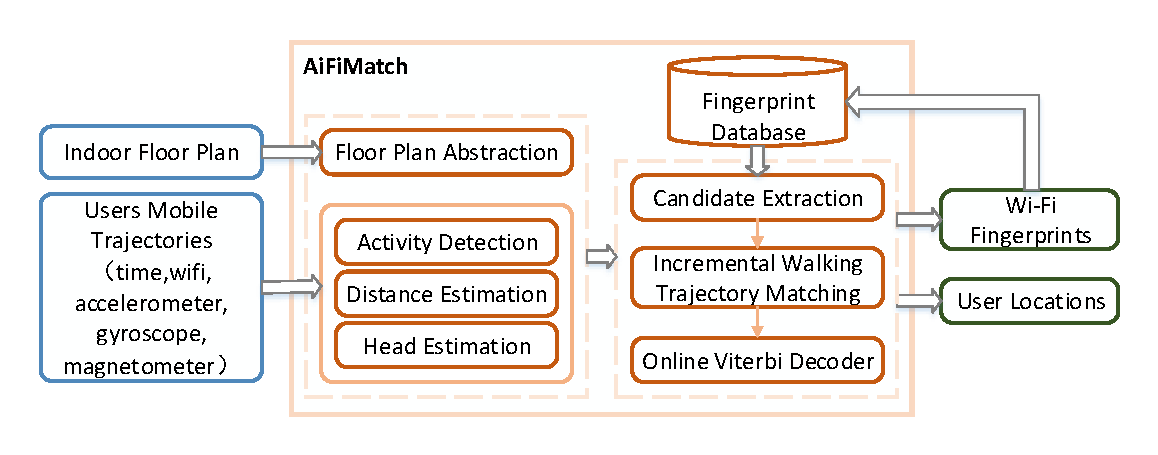
\includegraphics[width=4.7in]{AiFiMatch-Architecture}
	\caption{AiFiMatch System Architecture.}
	\label{fig-architecture}
\end{figure}
\vspace{-10pt}

Firstly, AiFiMatch starts by indoor floor plan abstraction to create a directed graph to facilitate the map matching model establishment. Secondly, the system estimates the walking distance and heading direction with data of motion sensors. Finally, location-related activities are detected with the pre-trained decision tree, and then the pedestrian's trajectory data including motion data and Wi-Fi RSS values are divided into trajectory subsets sequence.  

The directed graph of indoor floor plan and walking trajectory subsets sequence are then passed to the HMM based map matching module whose outputs include the pedestrian position estimations and Wi-Fi fingerprints. These Wi-Fi fingerprints can be used to update indoor radio map. Our HMM-based map matching module contains three sub-modules: Candidate Extraction, Incremental Walking Trajectory Matching and an Online Viterbi Decoder. The Candidate Extraction module determines the candidate road segments from the directed graph of indoor floor plan that satisfy the spatial and Wi-Fi signal conditions. The module takes into account the errors of pedestrian heading direction estimation and the previous bound Wi-Fi fingerprint. The Incremental Walking Trajectory Matching module integrates a number of modifications to the standard HMM based map matching algorithm to take walking trajectory subsets sequence into account as well as the detected activities to enhance the accuracy of the estimated indoor road paths. Finally, the Online Viterbi Decoder uses dynamic programming to efficiently determine the most probable indoor road segments sequence.

\subsection{Preprocessing}

In this section, we give the details of three preprocessing components and leave the details of the map matching and Wi-Fi enhancement algorithm to the next section.

\subsubsection{PDR Implementation Based on Smartphone:}

PDR is a positioning scheme that derives the current position by adding the estimated displacement to the previous one based on motion sensors carried by smartphones. In PDR scheme, the pedestrian's position is usually updated by the step and the heading direction during one step is supposed to be unchanged. The pedestrian's position after $k-1$ steps can be denoted as $(x_{k-1},y_{k-1})$. The $k$-th step length and heading direction are denoted as $sl_k$ and $\theta_k$, respectively. Then, the pedestrian's position after $k$ steps can be obtained by the following equation:
\begin{equation}
\label{equ_pdr}
\left( {\begin{array}{*{20}{c}}
	{{x_k}}\\
	{{y_k}}
	\end{array}} \right){\rm{ = }}\left( {\begin{array}{*{20}{c}}
	{{x_{k - 1}} + s{l_k} \cdot \sin {\theta _k}}\\
	{{y_{k - 1}} + s{l_k} \cdot \cos {\theta _k}}
	\end{array}} \right)
\end{equation}

%\begin{equation}
%\label{equ_pdr}
%({x_k},{y_k}) = ({x_{k - 1}} + s{l_k} \cdot sin{\theta _k},{y_{k - 1}} + s{l_k} \cdot \cos {\theta _k})
%\end{equation}

The heading direction is measured by the fusion of gyroscope and magnetometer. The step length and step count estimate approach is out of scope of this paper and can be found in \cite{wang2012no}. 

\subsubsection{Activity Detection:}

\vspace{-20pt}
\begin{figure*}[!ht]
	\centering
	\subfloat[$Decision\ Tree\ for\ Activity\ Detection $]{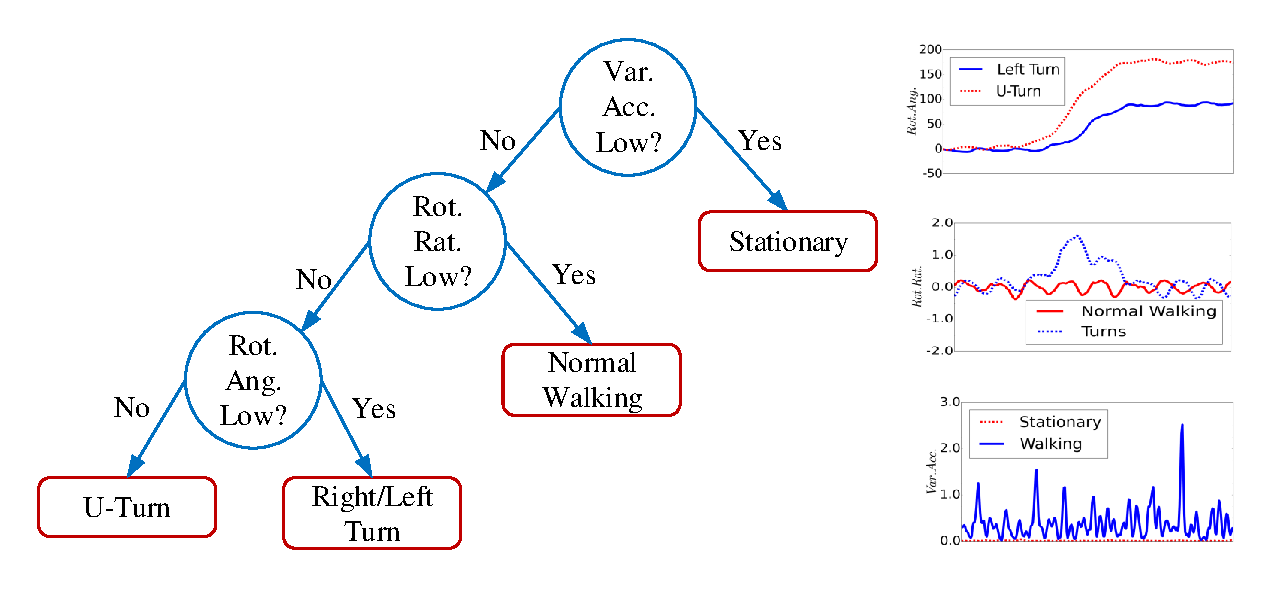
\includegraphics[width=4.75in]{AiFiMatch-ActivityDecision}%
		\label{fig-activity}}
	\vfil
	\subfloat[$Turning\ Activity\ Detected\ Example$]{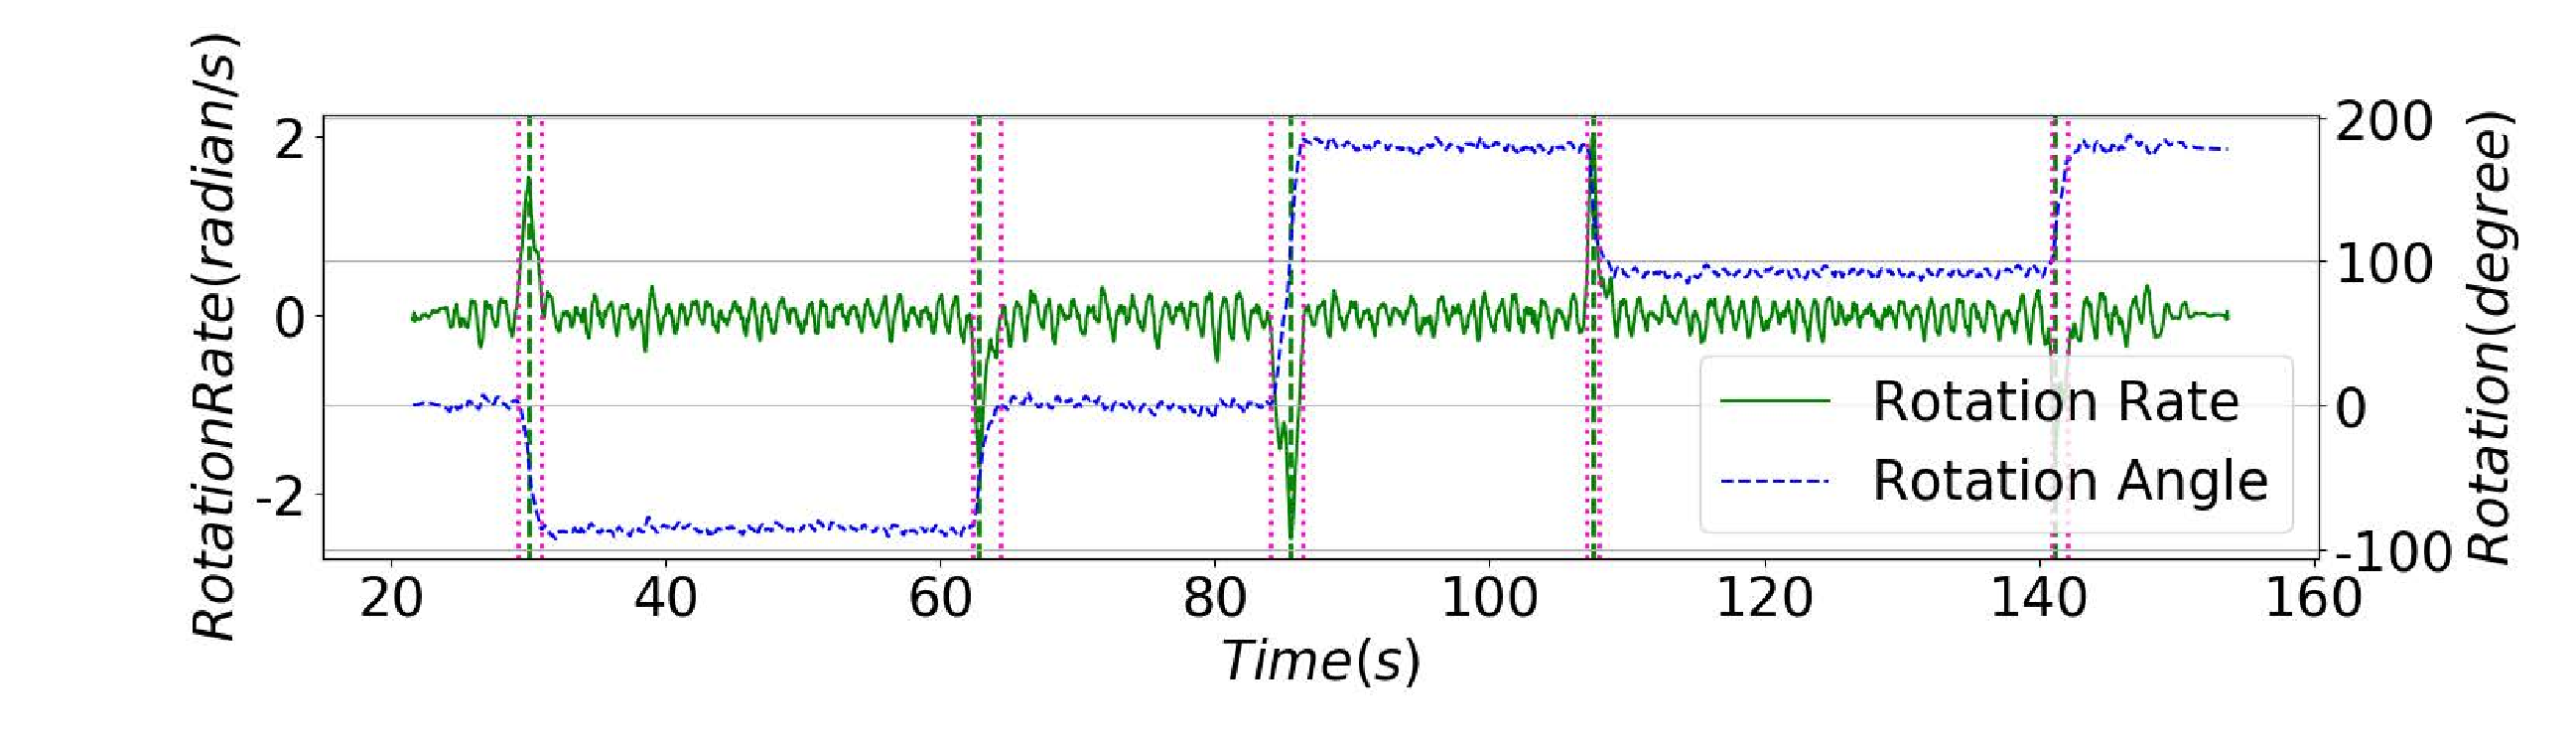
\includegraphics[width=4.85in]{AiFiMatch-TurnDemo}%
		\label{fig-turndemo}}
	\caption{Decision Tree for Activity Detection and An Example}
\end{figure*}
\vspace{-10pt}

In this paper, AiFiMatch considers four types of pedestrian activities: stationary, normal walking, turning at a corner (left or right turn) and turning around (U-turn), which would occur on the flat ground. The decision tree for activity detection and signal features of each activity is shown in Fig. \ref{fig-activity}. The top level separates walking and stationary based on the variance of the accelerometer. With the help of gyroscope, the second level uses the rotation rate to separate the normal walking and turns while the third level separates the U-turn case from the left or right turn case based on the rotation angle during the turning. Three participants with different brands of smartphones were asked to complete three activities (U-turn, left and right turn) in our experimental environment. The sample size of each activity was $60$ traces. Fig. \ref{fig-turndemo} shows an example for turning activity detection and the activity detection result is summarized in Table $1$.

\vspace{-10pt}
\begin{table}
	\label{table_conf}
	\caption{Confusion Matrix of Activity Detection}
	\begin{center}
		\begin{tabular}{| c || c | c | c | c |}
			\hline
			\bfseries Activity Type & \bfseries Left Turn & \bfseries Right Turn & \bfseries U-turn & \bfseries No Type\\
			\hline\hline
			\bfseries Left Turn & 58 & 0 & 0 & 2 \\
			\hline
			\bfseries Right Turn & 0 & 59 & 0 & 1 \\
			\hline
			\bfseries U-turn & 0 & 0 & 60 & 0 \\
			\hline
		\end{tabular}
	\end{center}
\end{table}
\vspace{-30pt}

\subsubsection{Indoor Floor Plan Abstraction:}

In the indoor environment, there are many activity-relative locations such as corridor corners and entrances of rooms where pedestrians may perform different activities other than normal walking. These special locations divide the indoor roads into segments. With road segments as nodes in the form of \emph{(coordinate of first endpoint $(x_1,y_1)$, accessible direction of first endpoint $({\varphi}_1)$, coordinate of second endpoint $(x_2,y_2)$, accessible direction of second endpoint $({\varphi}_2)$)}, the activity type from one road segment to another as directional edges in the form of \emph{(Activity Type (AT))}, the indoor floor plan would be represented as a direction graph. Fig. \ref{fig-abstract} shows an example of indoor floor abstraction. 

\vspace{-10pt}
\begin{figure}[!htbp]
	\centering
	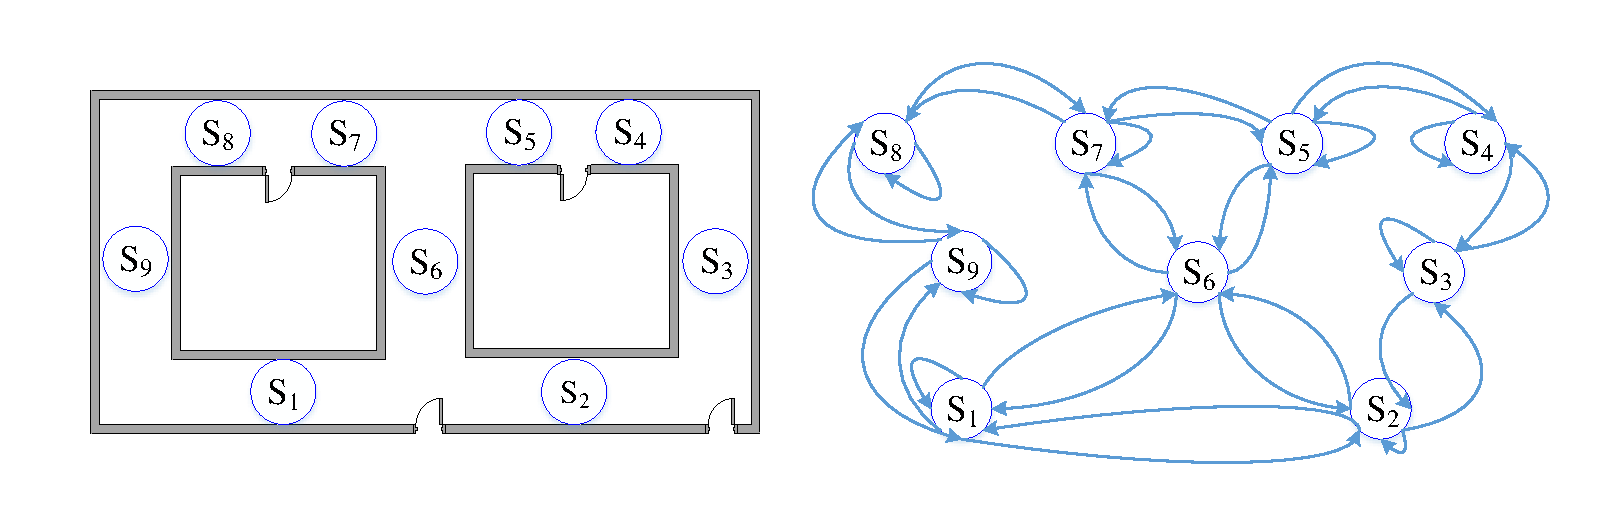
\includegraphics[width=4.576in]{AiFiMatch-MapAbstract}
	\caption{Floor Plan Abstraction Example.}
	\label{fig-abstract}
\end{figure}
\vspace{-20pt}

\section{HMM based Map Matching Algorithm}

Through this section, we detail the HMM-based map matching module of AiFiMatch system. We first start by providing the novel HMM model and the details of its components. Then, we describe the Wi-Fi enhancement algorithm for our proposed HMM model.

\subsection{Hidden Markov Model}

Taking computing power and energy limit of a smartphone into account, our proposed map matching algorithm select HMM to match the pedestrian's trajectory subsets sequence to the directed graph of indoor floor plan. A HMM can be represented as $\lambda  = (S,V,A,B,\pi)$, where:

1) $S = \left\{ {{s_1},{s_2},{s_3}, \ldots ,{s_N}} \right\}$ is the set of possible states and $N = \left| S \right|$. In our case, each state represents an indoor road segment, that is, a node of the directed graph. Therefore, a state $s$ is represented by the ordered tuple in the form of ($id,x_{1},y_{1},{\varphi}_{1},x_{2},y_{2},{\varphi}_{2}$), where $id$ is the identification of road segment, $x_{1}$, $y_{1}$, ${\varphi}_{1}$, $x_{2}$, $y_{2}$ and ${\varphi}_{2}$ are different attributes of node of the directed graph, respectively. $s.leng$ denotes the length of road segment and can be obtained from the coordinates of two endpoints of this road segment. \emph{Note that two or more road segments connected by a straight line can form new states (Fig. \ref{fig-viterbi}).}

2) $V = \left\{ {{v_1},{v_2},{v_3}, \ldots ,{v_M}} \right\}$ is the set of observations from the model and $M = \left| V \right|$. For each walking trajectory of a pedestrian, PDR technique gives displacement and heading direction estimations. However, due to the interference of many kinds of metal materials to the magnetic field in buildings, the heading direction estimation has a large error. Therefore, in our case, each observation is a displacement estimation and is represented by \emph{(dist)}.

3) $A = \left\{ {{a_{ij}}} \right\}$ is the state transition probability distribution, where \\ ${a_{ij}} = p\left\{ {{q_{t + 1}} = {s_j}|{q_t} = {s_i}} \right\}, i, j \le N$, where ${q_t}$ denotes the state at time $t$. In our case, the transition probability $a_{ij}$ is the probability of walking to the next road segment $s_{j,t}$ given the current road segment is $s_{i,t-1}$. Intuitively, for probable transition between two road segments, the pedestrian's activity should match the activity type between the same two segments. Therefore, given the detected activity of a pedestrian ${Ped_{AT}}(t)$ at time $t$ and the activity type between two segments ${Seg_{AT}}^{ij}$, AiFiMatch models this intuition by the equation \ref{equ_transition}, where $p({Ped_{AT}}(t)|{Seg_{AT}}^{ij})$ can be found in confusion matrix.
\begin{equation}
\label{equ_transition}
p({s_{j,t}}|{s_{i,t - 1}}) = p({s_j}|{s_i},{Ped_{AT}}(t)) = p({Ped_{AT}}(t)|{Seg_{AT}}^{ij})
\end{equation}

4) $B = \left\{ {{b_i}(k)} \right\}$ is the observation probability distribution in state $i$, where ${b_i}(k) = p\{ {o_t} = {v_k}|{q_t} = {s_i}\},1 \le i \le N,1 \le k \le M$ and $o_t$, $q_t$ are the observation and state at time $t$, respectively. Observation probabilities also called emission probabilities represent the likelihood that a measurement resulted from a given state. In our case, given a displacement observation ${v_k}.dist(t)$, there is an emission probability $p({v_k}.dist(t)|{s_i}.leng)$ for each candidate road segment $s_i$, where ${s_i}.leng$ denotes the length of road segment $s_i$ which can be obtained from the coordinates of two endpoints of this road segment. If a pedestrian has passed the complete road segment $s_i$, AiFiMatch models the emission probability as a Gaussian Distribution:
\begin{equation}
\label{equ_emission1}
{f_1}({\rm{v_k}}{\rm{.dist(t),}}{{\rm{s}}_{\rm{i}}}{\rm{.leng}}) = \frac{1}{{\sqrt {2\pi } {\sigma _d}}}{e^{ - \frac{{{{({v_k}.dist(t) - {s_i}.leng)}^2}}}{{2{{\sigma}_d}^2}}}}
\end{equation}

where ${\sigma}_d$ is the standard deviation of the measured displacement. Based on the distance calculation method of PDR, the displacement is in direction proportion to step length. Therefore, ${\sigma}_d$ can be obtained based on the standard deviation of step length ${\sigma}_s$. Considering the situation that a pedestrian is walking on the road segment, all long enough candidate road segments should have the same probability, AiFiMatch models the situation using the equation as:
\begin{equation}
{f_2}({\rm{v_k}}{\rm{.dist(t),}}{{\rm{s}}_{\rm{i}}}{\rm{.leng}}) = \frac{1}{{\sqrt {2\pi } {\sigma _d}}}{e^{-4.5}},{v_k}.dist(t) + 3{\sigma _d} \le {s_i}.leng
\end{equation}

Hence, the final emission probability, $p(v_k|s_i)$, is modeled as:
\begin{equation}
p(v_k|s_i)=f({v_k}.dist(t),{s_i}.leng) = \left\{ {\begin{array}{*{20}{l}}
	{\frac{1}{{\sqrt {2\pi } {\sigma _d}}}{e^{-4.5}},{v_k}.dist(t) + 3{\sigma _d} \le {s_i}.leng}\\
	{\frac{1}{{\sqrt {2\pi } {\sigma _d}}}{e^{ - \frac{{{{({v_k}.dist(t) - {s_i}.leng)}^2}}}{{2{\sigma _d}^2}}}},otherwise}
	\end{array}} \right.
\end{equation}

5) $\pi  = \left\{ {{\pi _i}} \right\}$ is the initial state distribution, where ${\pi _i} = p\left\{ {{q_1} = {S_i}} \right\},1 \le i \le N$. If the starting point or the first road segment is known, the initial state distribution is $1$ since the first road segment is the only candidate; otherwise, all candidate road segments are selected by the \emph{Candidate Extraction} module and the initial state distribution is uniform in all candidates. Let $S_c$ denote the set of all candidates, and the initial state distribution is re-estimated after each step by the equation \ref{equ_initupdate} until the first location-related activity is detected.
\begin{equation}
\label{equ_initupdate}
{\pi _{i,t}} = {\pi _{i,t - 1}} \cdot f({v_k}.dist(t),{s_i}.leng),{s_i} \in {S_c}
\end{equation}

\subsection{Candidate Extraction}

AiFiMatch uses the heading direction of a pedestrian and Wi-Fi fingerprint to select the candidate states. Here, we describe the extraction algorithm by heading direction and leave the Wi-Fi fingerprint extraction algorithm to the \emph{Wi-Fi Enhancement} Section.
	 
Intuitively, the heading direction of a pedestrian should match the direction of road segment. Therefore, AiFiMatch models the direction difference by the following function to select the candidates:
\begin{equation}
{g_1} = {g_1}({Ped_{dir}},s) = \left\{ {\begin{array}{*{20}{l}}
	{1,if\left| {{Ped_{dir}} - s.{{\varphi}_j}} \right| < H_{TH},j = 1,2}\\
	{0,otherwise}
	\end{array}} \right.
\end{equation}

where $Ped_{dir}$ denotes the heading direction of a pedestrian, $s$ is a state, $H_{TH}$ is the threshold for candidate extraction, which is set to \emph{55 (degree)} based on the experiments.

\subsection{Wi-Fi Enhancement}
Map matching offers an important source of information and an excellent way to improve the position estimations, especially in narrow corridors, but it has some limitations when the indoor environment presents symmetries that generates multiple hypotheses. Supposing that a pedestrian walks along this segments sequence $(s_3, s_4, s_5, s_6)$, as shown in Fig. \ref{fig-viterbi}, for the given observable states, it is directly to be seen that the segments sequence $(s_6, s_7, s_8, s_9)$ may have almost the same matching probability as the actual one. In this situation, traditional HMM based map matching algorithm fails \cite{zhou2015activity}.

\vspace{-10pt}
\begin{figure}[!htbp]
	\centering
	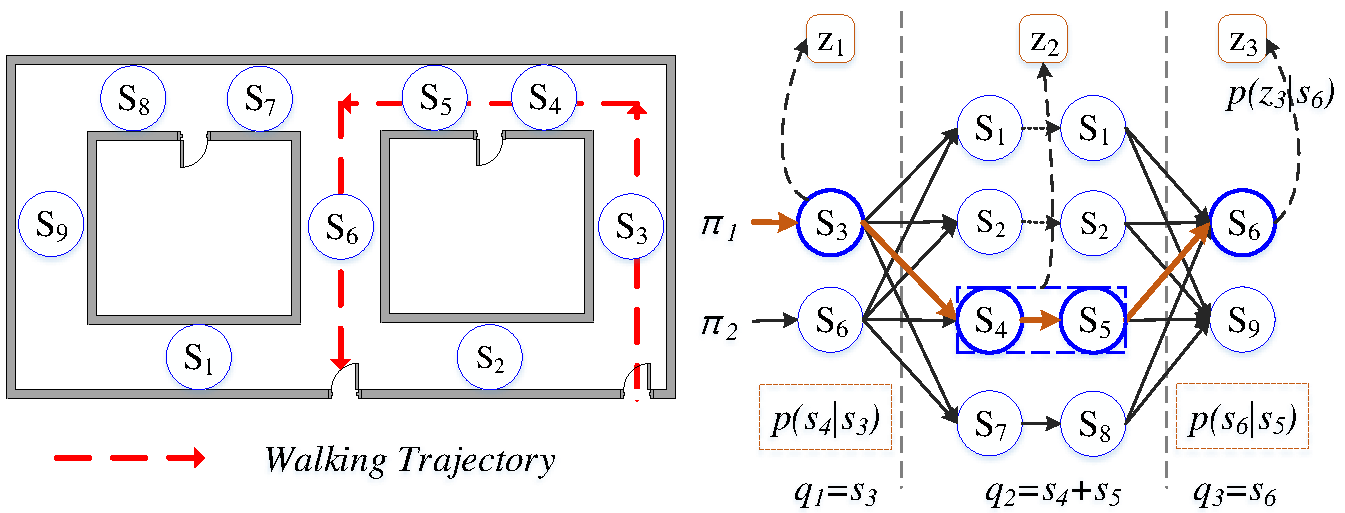
\includegraphics[width=4.6in]{AiFiMatch-Viterbi}
	\caption{Illustration of the Viterbi Decoding.}
	\label{fig-viterbi}
\end{figure}
\vspace{-10pt}

AiFiMatch introduces Wi-Fi dissimilarity to distinguish multiple hypotheses due to the symmetry of building structure. After AiFiMatch determines a pedestrian's walking trajectory by the Online Viterbi Algorithm \cite{aly2015semmatch}, the pedestrian's positions can be derived by PDR using the two endpoints of determined segments as the starting point. Therefore, Wi-Fi fingerprints collected synchronously during the pedestrian walking can be bound to the corresponding positions by time alignment and then update the Wi-Fi fingerprint database of indoor environment where the pedestrian is located. In order to improve the HMM based map matching algorithm described above, the paper not only binds Wi-Fi fingerprints to physical positions but also road segments. All Wi-Fi fingerprints of one road segment are sorted in the road segment's direction. For two fingerprints $f_x$, $f_y$, and MAC address set of their Access Points $X$, $Y$, define dissimilarity $J_{\delta}$ between $f_x,f_y$ as follows:
\begin{equation}
{J_\delta }(f_x,f_y) = 1 - J(X,Y) = \frac{{|X \cup Y| - |X \cap Y|}}{{|X \cup Y|}}
\label{equ-jad}
\end{equation}

where equation \ref{equ-jad} is known as Jaccard distance. With this dissimilarity of two fingerprints, we define the similarity function $L(S_a, S_b)$ between two fingerprint sequences $S_a = (f_1^a,f_2^a,\cdots,f_w^a)$, $S_b = (f_1^b, f_2^b, \cdots, f_k^b)$:
\begin{equation}
\begin{array}{c}
L({S_a},{\rm{ }}{S_b}) = \min (\frac{1}{w}\sum\limits_{t = 1}^w {{J_\delta }({f_t}^a,{f_{i + t}}^b),0 \le i \le k - w,} \\
\frac{1}{w}\sum\limits_{t = 1}^w {{J_\delta }({f_t}^a,{f_{j - t}}^b),w + 1 \le j \le k + 1} )
\end{array}
\end{equation}

where $w=|S_a|$, $k=|S_b|$ and $2<w<k$. Given segment candidate set $G$ and the set $R$ of all road segments bound with Wi-Fi fingerprints sequence, Finally, AiFiMatch models the dissimilarity of two Wi-Fi fingerprint sequences and the different stages of fingerprint database by the following function to select the candidates: 
\begin{equation}
{g_2} = {g_2}({S_{ped,}}{S_i}) = \left\{ {\begin{array}{*{20}{l}}
	{0,if{\kern 1pt} i{\kern 1pt}  \ne \mathop {\arg \min }\limits_j \{ L({S_{ped,}}{S_j}),{S_j} \in G,G \subseteq R\} }\\
	{0,if{\kern 1pt} \min \{ L({S_{ped}},{S_i}),{\kern 1pt} {\kern 1pt} {S_i} \in G{\kern 1pt} {\kern 1pt}  \cap R\}  > d{\kern 1pt} {\kern 1pt} }\\
	{1,otherwise}
	\end{array}} \right.
\end{equation}

where $d$ is the threshold to distinguish two Wi-Fi fingerprint sequences. 

A pilot study is conducted to evaluate the dissimilarities between two fingerprint sequences of same and different road segments. A prototype installed in three smartphones (360 N5, OPPO R827T and Xiaomi 3W) is used to collect Wi-Fi RSS values at $1$Hz. Each participant was asked to walk along two symmetric road segments in two directions. The participant with 360 N5 smartphone was asked to repeat $12$ times while the others were asked to repeat $6$ times. Among them, $6$ Wi-Fi data collected by 360 N5 smartphone were used as Wi-Fi fingerprint database, while other Wi-Fi data were used as online Wi-Fi fingerprint sequences. The maximum and minimum dissimilarities between fingerprint sequences of same and different road segments are shown in Fig. \ref{fig-wifidist}. From Fig. \ref{fig-wifidist}, with increases in the length of Wi-Fi fingerprint sequence $w$, the dissimilarity between two sequences of same segments gradually decreases, while the dissimilarity between two sequences of different segments gradually increases. Considering the device diversity, in order to avoid missing the correct alternative segments, the minimum value of the threshold $d$ is $0.773$.

\vspace{-10pt}
\begin{figure}[!htbp]
	\centering
	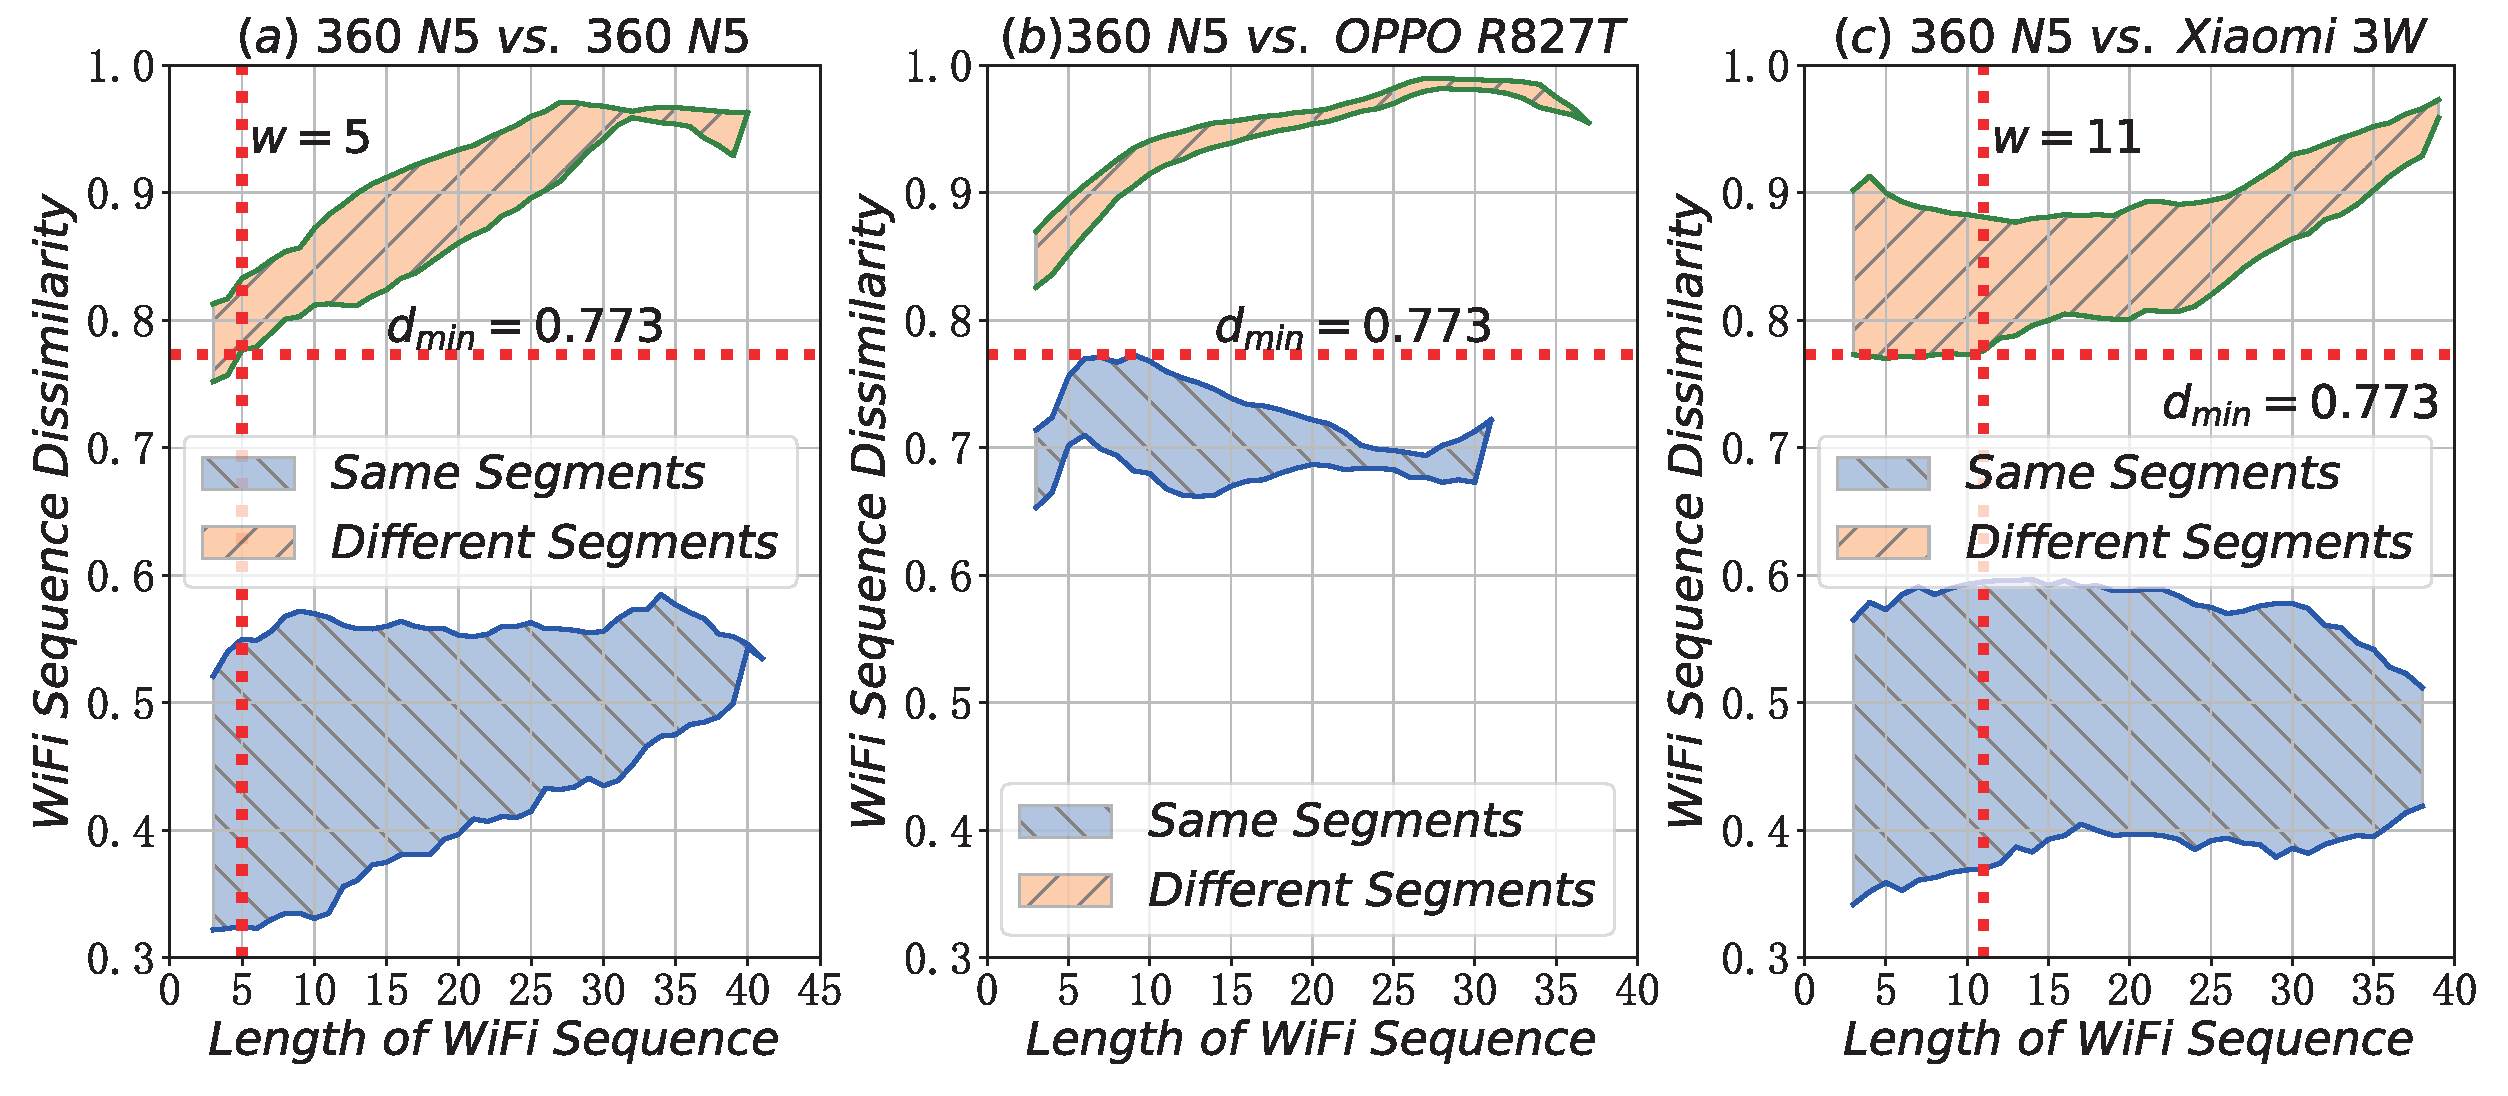
\includegraphics[width=4.94in]{AiFiMatch-WiFiJCD}
	\caption{Dissimilarity between Two Wi-Fi Fingerprint Sequences from Multiple Devices.}
	\label{fig-wifidist}
\end{figure}
\vspace{-20pt}

\subsection{Optimal State Sequence Estimation}

Once the HMM parameters are estimated, we can use the Viterbi algorithm to get the most probable hidden states sequence $Q = ({q_1},{q_2},...,{q_k})$ for a given observation sequence $O = ({o_1},{o_2},...,{o_k})$. A Viterbi variable ${\delta _t}(i)$ is defined by equation \ref{equ-vtbvar} to represent that, at time $t$, the HMM model reaches the hidden state $s_i$ along a certain path and outputs the maximum probability.
\begin{equation}
	\label{equ-vtbvar}
	{\delta _t}(i) = max\{ p({q_1},{q_2},...,{q_t} = {s_i},{o_1},{o_2},...,{o_t}|\lambda )\}
\end{equation}

At time $t+1$, the maximum probability reaching the hidden state $s_j$ can be recursively derived from the Viterbi variable at time $t$ by the following equation. 
\begin{equation}
	{\delta _{t + 1}}(j) = [\mathop {max}\limits_i \{ {\delta _t}(i) \cdot p({q_{t + 1}} = {s_j}|{q_t} = {s_i})\} ] \cdot p({o_{t + 1}}|{q_{t + 1}}),1 \le t \le k
\end{equation}

For AiFiMatch to operate in real-time, it cannot wait until the whole sequence is available. Hence, The online Viterbi algorithm \cite{bloit2008short} is applied to compute the maximum likelihood sequence of states using dynamic programming. AiFiMatch uses Viterbi algorithm in an incremental manner. Every time a new step of a pedestrian is detected, the HMM parameters are calculated for the new introduced sensors data and the associated candidate states.  Fig. \ref{fig-viterbi} illustrates the proposed HMM model Viterbi decoding. The decoded sequence is colored in blue.

During the beginning process of the algorithm, if the number of states is too small, the most probable states sequence is not always the correct one, especially when the starting point of pedestrian is unknown. Therefore, we give a criteria by the equation $c = {{{p_{fir}}} \mathord{\left/
		{\vphantom {{{p_{fir}}} {{p_{\sec }}}}} \right.
		\kern-\nulldelimiterspace} {{p_{\sec }}}}$ to determine the status of this algorithm, where ${p_{fir}}$ is the highest probability of the states sequence and ${p_{\sec }}$ is the second highest probability of the states sequence. We set a threshold, if $c$ is greater than or equal to the threshold, we choose the Viterbi decoding result. The selected hidden states sequence represents the pedestrian's passed indoor road segments.

AiFiMatch algorithm is summarized with the pseudocode in Algorithm \ref{alg_aifi}.  

\vspace{-10pt}
\begin{algorithm}[H]
	\caption{AiFiMatch online map matching algorithm}
	\label{alg_aifi}
	\begin{algorithmic}[1]
		\renewcommand{\algorithmicrequire}{\textbf{Input:}}
		\renewcommand{\algorithmicensure}{\textbf{Output:}}
		\REQUIRE Sensor data up to current time t: $data_{1:t}$
		\REQUIRE Abstract Indoor Floor Plan: $fp$
		\REQUIRE Hidden State Sequence and Its Length up to last time $t-1$: $S_{k}(t-1)$, $k$
		\REQUIRE Array of Viterbi variable and backward pointer: ${VtbArr}_{k}(t-1)$
		\ENSURE Pedestrian's position estimation at current time $t$: $Ped_{loc}(t)$
		\ENSURE Optimal state sequence estimation at current time $t$: $Q(t)$
		\STATE ${Ped_{AT}(t)}, at \leftarrow activity\_detect({data_{1:t}})$
		\IF{$Ped_{AT}(t)\ != \ None$}  
		\STATE ${st} \leftarrow {at}$  
		
		\STATE // Calculate the transition probability
		\STATE $S(t) \leftarrow [\ ]$
		\FOR{$s_i\ \in\ S_{k}(t-1)$}
		\STATE // Select next segments according to $fp$
		\STATE $S^{i}(t) \leftarrow next(fp,s_i)$
		\STATE // Extract segments according to Wi-Fi data
		\STATE $S^{i,wifi}(t) \leftarrow extract(data_{st:t}^{wifi},S^{i}(t))$
				
		\algstore{myalg}
	\end{algorithmic}
\end{algorithm}
		
\begin{algorithm}[t]
	\begin{algorithmic}[1]
		\algrestore{myalg}		

		\FOR{$s_j\ \in\ S^{i,wifi}(t)$}
		\STATE $tr[i][j] \leftarrow p(s_j|s_i,{Ped_{AT}(t)})$
		\ENDFOR
		\STATE $S(t).extend(S^{i,wifi}(t))$
		\ENDFOR
		
		\STATE // Calculate the observation probability		    
		\STATE ${z_t} \leftarrow dead\_reckon(data_{st:t})$
		\FOR{$s_i\ \in\ S(t)$}
		\STATE $ob[i]\ \leftarrow\ p(z_t|s_i)$
		\ENDFOR
		\STATE ${VtbArr}_{k+1}(t) \leftarrow viterbi({VtbArr}_{k}(t-1), ob[\ ], tr[\ ][\ ])$
		\STATE $k \leftarrow k+1$
		\STATE $S_{k}(t) \leftarrow S(t)$
		
		\ELSE // Not a location-related activity
		\STATE $ob \leftarrow [\ ],\ S_{k}(t) \leftarrow S_{k}(t-1)$
		\STATE // Update the observation probability
		\STATE ${z_t}=dead\_reckon(data_{st:t})$
		\FOR{$s_i\ \in\ S_{k}(t)$}
		\STATE $ob[i]\ \leftarrow\ p(z_t|s_i)$
		\ENDFOR
		\STATE ${VtbArr}_{k}(t) \leftarrow viterbi({VtbArr}_{k}(t-1), ob[\ ])$
		\ENDIF	
		
		\STATE // Optimal State Sequence
		\STATE ${Q(t)} \leftarrow None$
		\IF{$check\_status(VtbArr^{k}(t))=Convergence$}
		\STATE ${Q(t)} \leftarrow viterbi\_decode(VtbArr^{k}(t))$
		\ENDIF
		
		\STATE // Update the location estimation according to $Q(t)$
		\STATE $Ped_{loc}(t) \leftarrow update\_location(data_{st:t}, Q(t))$
	\end{algorithmic}
\end{algorithm}
\vspace{-10pt}


\section{Evaluation}

\subsection{Environment Setup}

In this section, we show our evaluation for the performance of AiFiMatch in real-world environment. We conduct experiments in the fifth floor of a teaching hall on campus. Approximately, we cover a $78.95m \times 56.40m$ floor plan, as shown in Fig. \ref{fig-envionment}. A prototype is implemented and installed on a 360 N5 Android version 6.0.1 smartphone, a OPPO R827T Android version 4.4.0 smartphone and a Xiaomi 3W Android version 6.0.1 smartphone. The prototype samples the accelerometer, gyroscope and magnetometer sensors at $50$Hz and Wi-Fi at $1$Hz. Three participants (two males and one female) were asked to complete the experiments. The participants were asked to walk along Trajectory $No.1$ ($T_1$), Trajectory $No.2$ ($T_2$) and Trajectory $No.3$ ($T_3$) at constant speed. Each trajectory was repeated six times by all participants. In order to record the walking trajectories, all the participants' shoes were painted with colored powder. This offered the ground truth.

\subsection{Performance of Map Matching}

To evaluate AiFiMatch map matching performance, we start by showing the online positioning performance of AiFiMatch and basic PDR technique. After that, we analyze the effect of step length and heading errors on positioning accuracy. Then, we discuss the convergence performance as compared to an activity sequence-based map matching algorithm proposed by \emph{Zhou et al} \cite{zhou2015activity}. Finally, we show the offline positioning results when using AiFiMatch.

\subsubsection{Online Positioning Performance:}

Euclidean distance between the estimated position and the ground truth is introduced to indicate positioning accuracy.  Fig. \ref{fig-online} shows the online positioning results of all trajectories for basic PDR algorithm with known initial point and AiFiMatch without known initial point.  Here, the mean position of all segment candidates' starting point is taken as initial point of AiFiMatch algorithm. Generally, for one trajectory, the greater the traveled distance, the larger the positioning error of PDR due to cumulative errors, Fig. \ref{fig-online} shows the trend.  However, after passing a number of steps, the traveled segment sequence determined by AiFiMatch even without known the initial point and the cumulative  errors are eliminated successfully.

\vspace{-10pt}
\begin{figure}[!htbp]
	\centering
	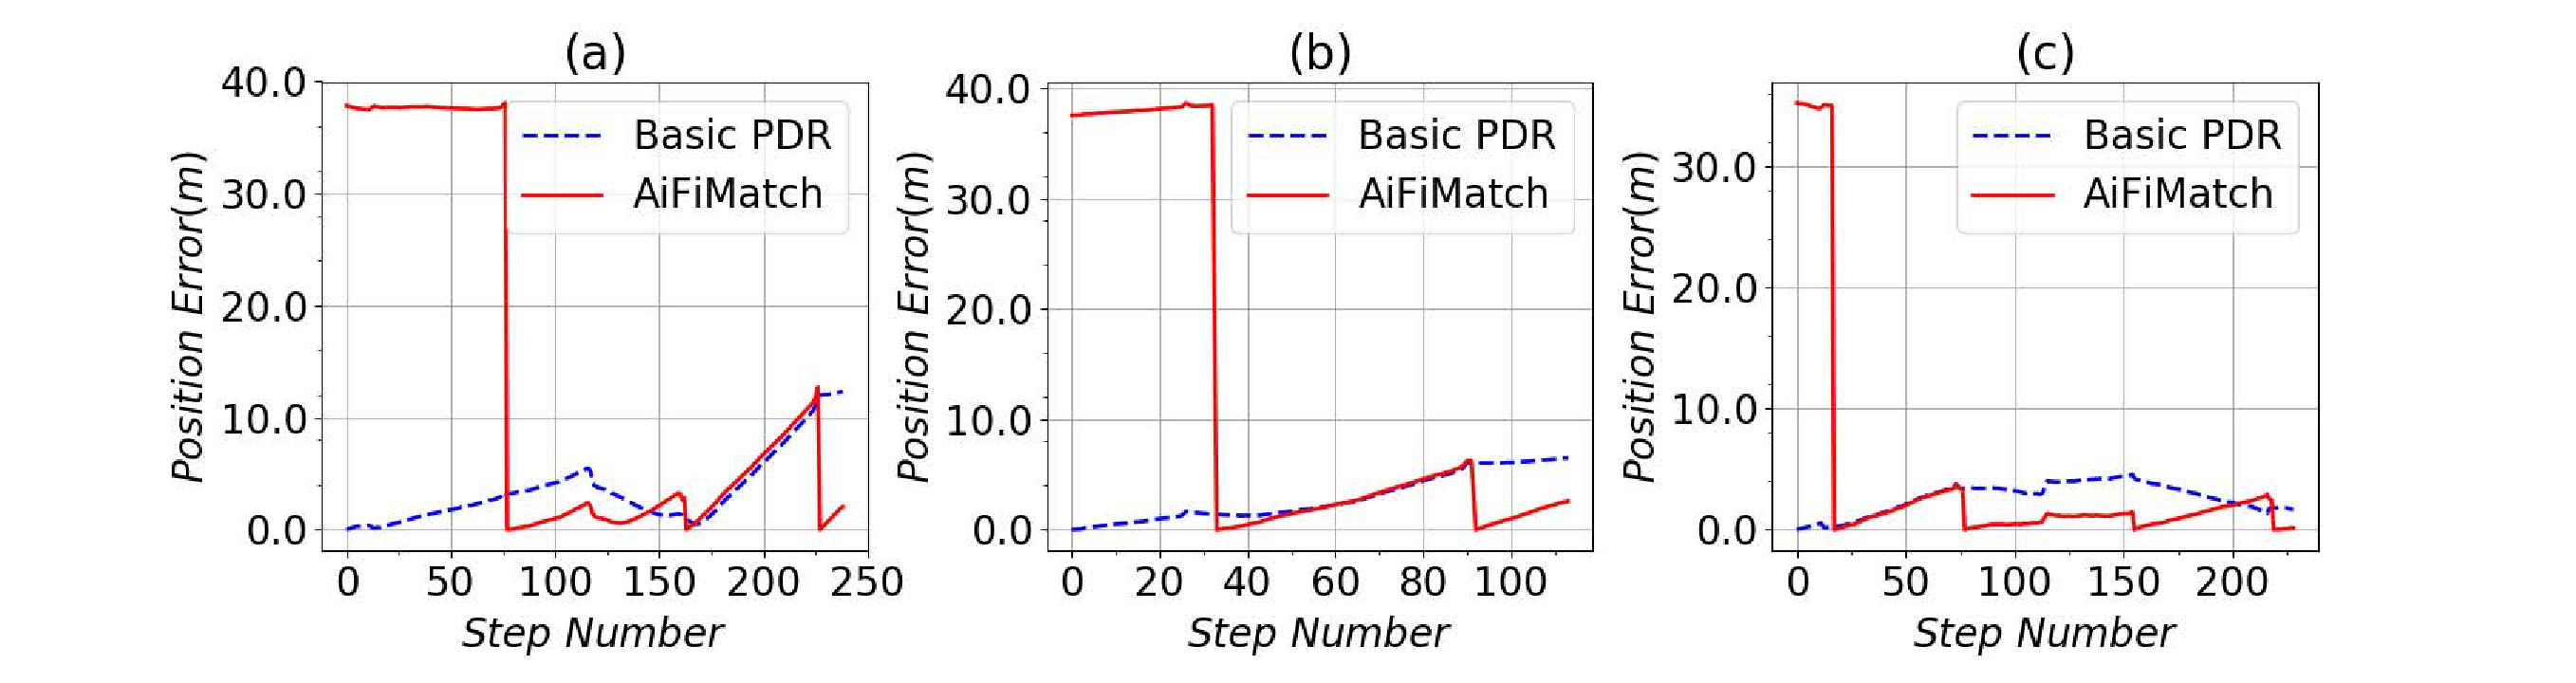
\includegraphics[width=4.8in]{AiFiMatch-OnlinePosition}
	\caption{Online Positioning Results for Each Trajectory. (a) $T_1$. (b) $T_2$. (c) $T_3$}
	\label{fig-online}
\end{figure}
\vspace{-10pt}

\subsubsection{Influence of Step Length and Heading direction Errors: }

The major errors of PDR techniques are mainly from step length and heading direction errors. Therefore, we analyze the influence of step length and heading direction errors to the average online positioning errors. Both of them are supposed to follow the Gaussian distributions with a mean zero. $\sigma_s$ denotes the standard deviation of step length estimation and $\sigma_{\varphi}$ denotes the standard deviation of heading direction estimation. When $\sigma_s$ changes from $0.1$ m to $0.5$ m, $\sigma_{\varphi}$ is set to $10$ degree. When $\sigma_{\varphi}$ changes from $10$ degree to $50$ degree, $\sigma_s$ is set to $0.1$ m. Fig. \ref{fig-errinfluence} shows the results of all trajectories with different errors. The performance of AiFiMatch in all error cases is superior to the basic PDR technique. From Fig. \ref{fig-errinfluence} \emph{(a)-(c)}, with increasing step length error, the average online positioning errors increases gradually. The same trend is shown in Fig. \ref{fig-errinfluence} \emph{(d)-(f)}, reflecting the influence of heading direction errors on the average online positioning errors. $T_1$ and $T_3$ have five location-related activities while $T_2$ has only two. As a result, given the same heading direction errors, the online positioning performance of AiFiMatch is more robust to $T_1$ and $T_3$ than $T_2$, which can also be seen from Fig. \ref{fig-errinfluence} \emph{(d)-(f)}.

\vspace{-10pt}
\begin{figure}[!htbp]
	\centering
	\includegraphics[width=4.56in]{AiFiMatch-ErrInfluence}
	\caption{Online Positioning Errors for Each Trajectory with Given Standard Deviations of Step Length and Heading Direction. (a) $T_1$. (b) $T_2$. (c) $T_3$. (d) $T_1$. (e) $T_2$. (f) $T_3$.}
	\label{fig-errinfluence}
\end{figure}
\vspace{-10pt}

\vspace{-10pt}
\begin{figure}[!htbp]
	\centering
	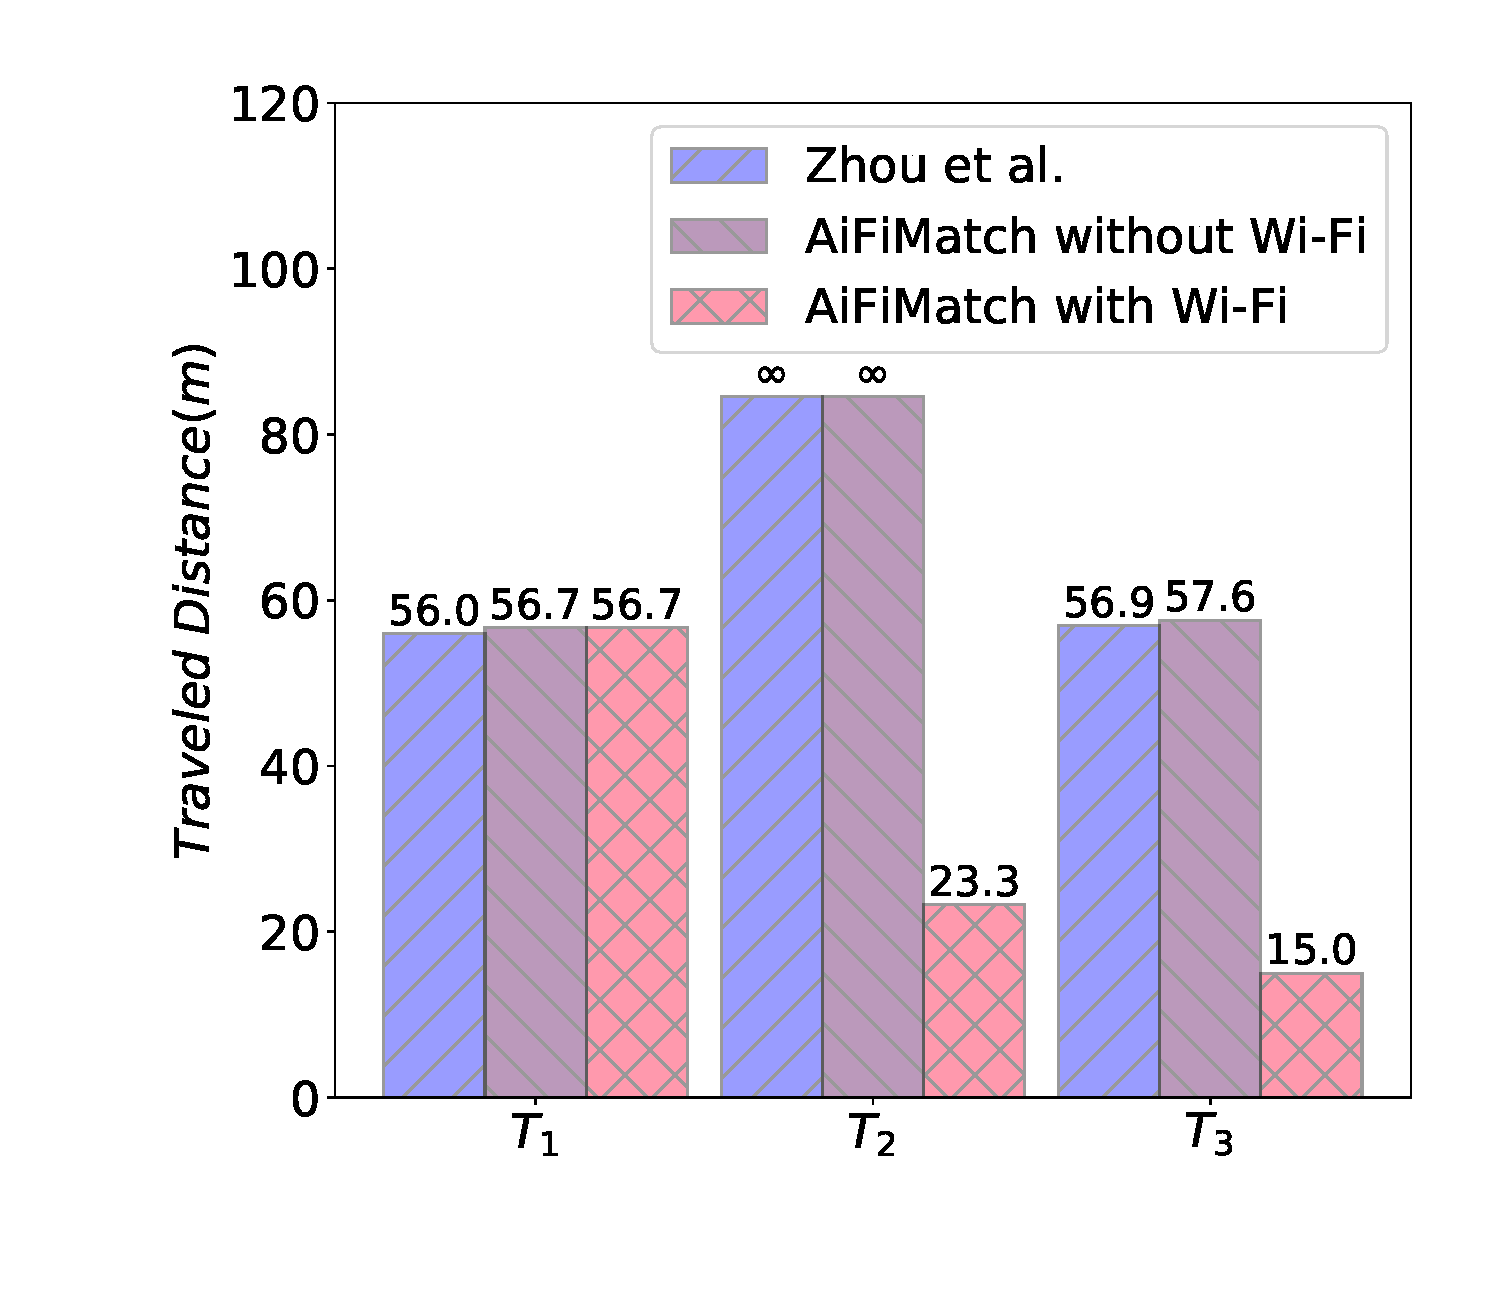
\includegraphics[width=2.3in]{AiFiMatch-Convergence}
	\caption{Distance traveled before convergence for each trajectory.}
	\label{fig-converg}
\end{figure}
\vspace{-10pt}

\subsubsection{Convergence Speed:}

We compare the performance of AiFiMatch algorithm in terms of convergence to map matching algorithm proposed by \emph{Zhou et al}. Distance traveled before converging to a unique states sequence reflects the convergence speed. The greater the traveled distance, the slower is the convergence speed. Fig. \ref{fig-converg} shows the traveled distance before convergence for \emph{Zhou et al}, AiFiMatch without Wi-Fi enhancement and AiFiMatch with Wi-Fi enhancement. At the initial stage, fingerprint database is empty ($T_1$), AiFiMatch and \emph{Zhou et al.} both successfully converge even without known the initial point. AiFiMatch without Wi-Fi enhancement and map matching algorithm proposed by \emph{Zhou et al.} fail to converge ($\infty$ means $T_2$ cannot be converged.) due to the symmetry of building structure. However, with the help of Wi-Fi signal, $T_2$ reaches convergence quickly. Mostly, with Wi-Fi enhancement, the traveled distance is much shorter than without Wi-Fi enhancement($T_2, T_3$). 



%\begin{figure}[!htbp]
%	\begin{minipage}[t]{0.5\textwidth}
%		\centering
%		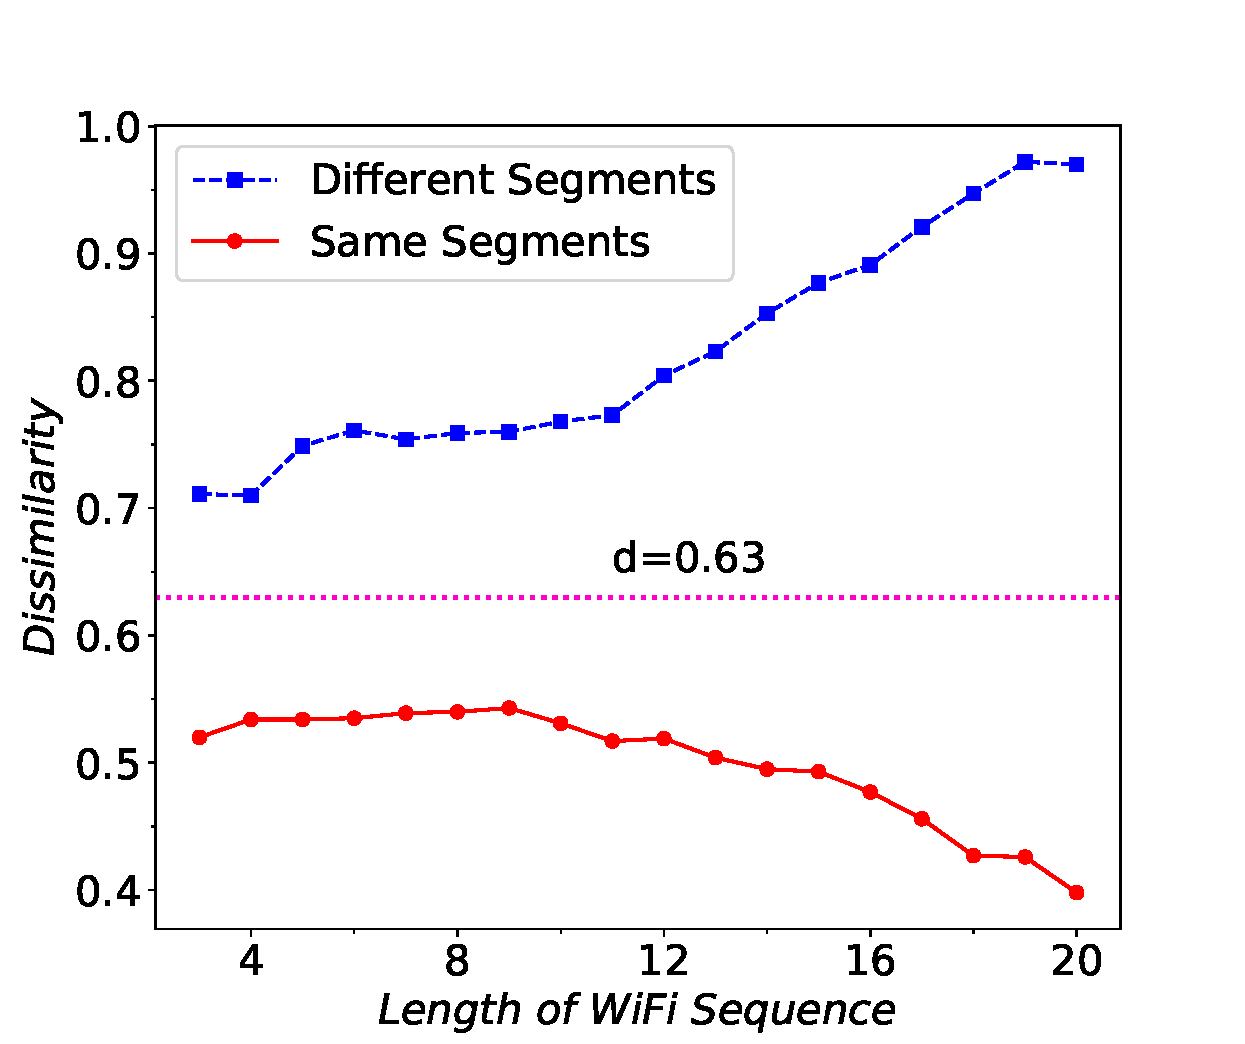
\includegraphics[width=2.58in]{AiFiMatch-WiFiDist}
%		\caption{Dissimilarity of Two Wi-Fi Fingerprint Sequences.}
%		\label{fig-wifidist}
%	\end{minipage}
%	\hfil
%	\begin{minipage}[t]{0.46\textwidth}
%		\centering
%		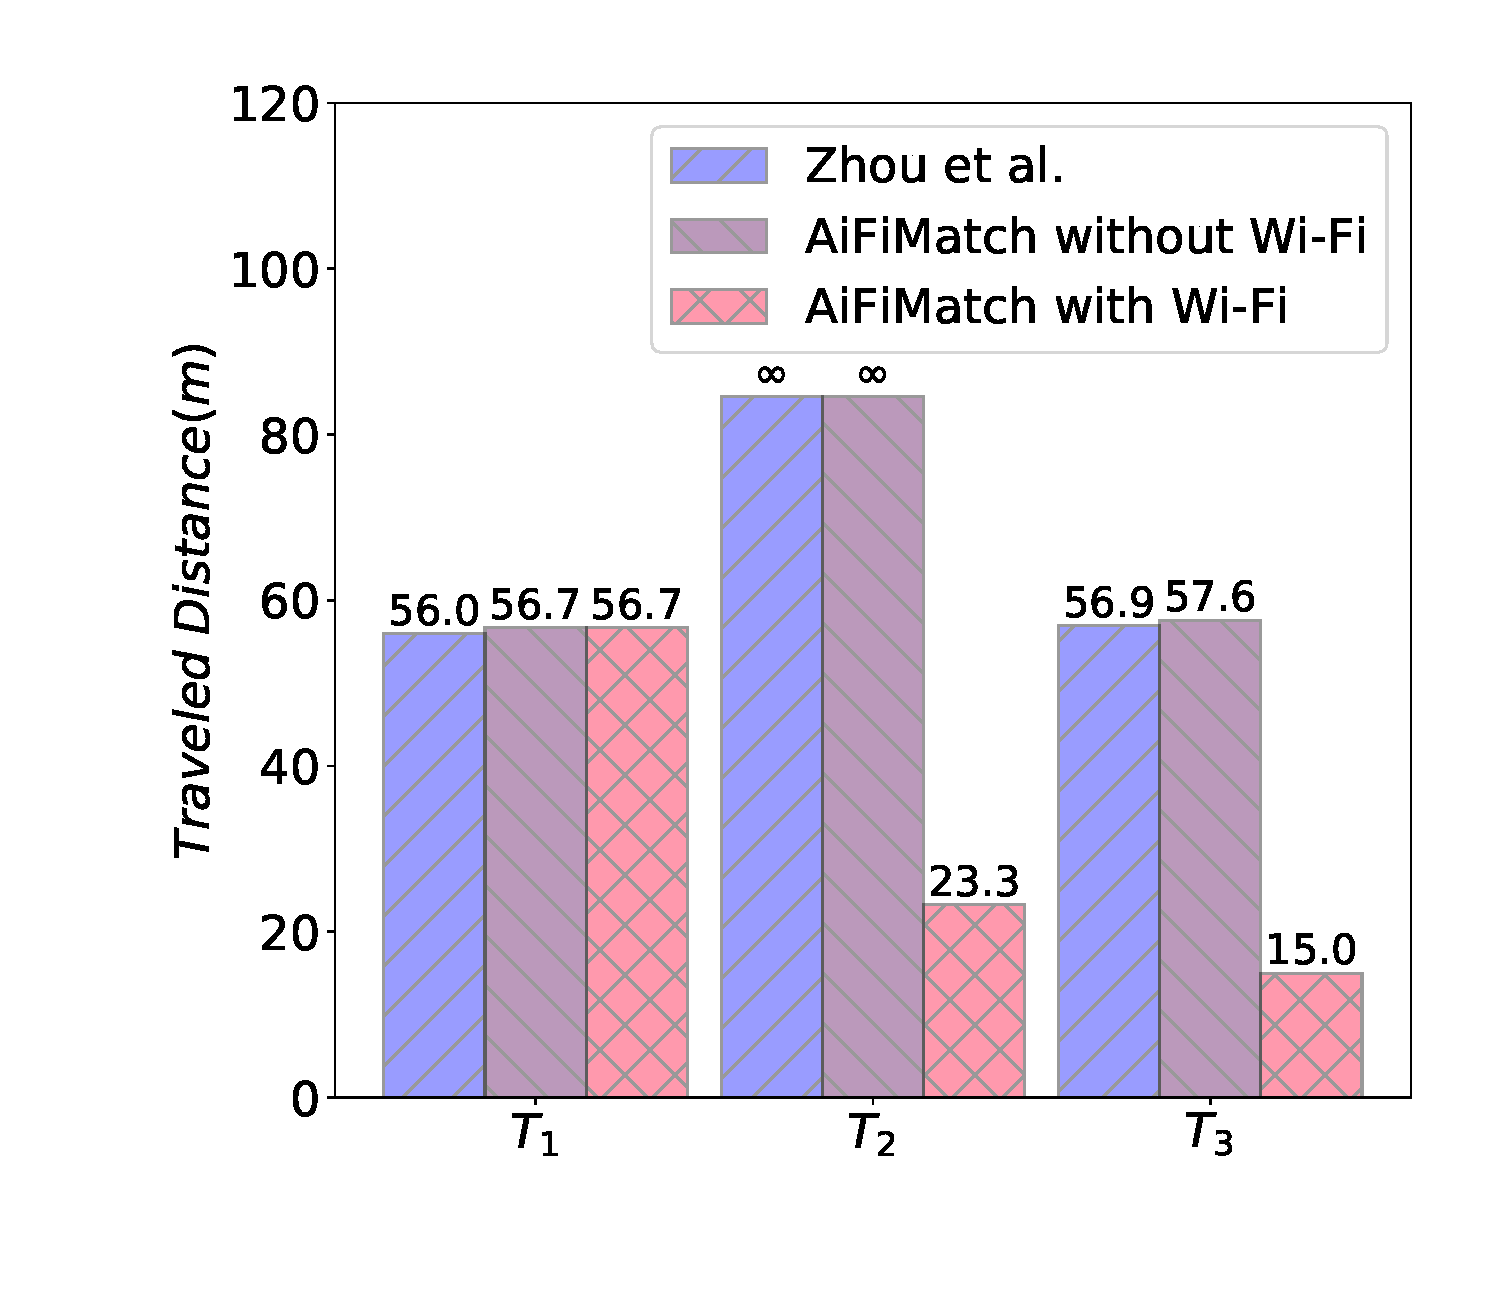
\includegraphics[width=2.3in]{AiFiMatch-Convergence}
%		\caption{Distance Traveled before Convergence for Each Trajectory.}
%		\label{fig-converg}
%	\end{minipage}
%\end{figure}



\subsubsection{Offline Positioning Performance:}

The offline positioning results are derived retrospectively after matching the walking trajectory of a pedestrian to a unique road segments sequence by AiFiMatch. Fig. \ref{fig-envandoffline} shows the tracking trajectories and some details are summarized in Table 2. AiFiMatch system tracked pedestrians' trajectories accurately in the experiment environments and the mean error of the offline positioning is about $1.24$ m.


\vspace{-10pt}
\begin{figure*}[!htbp]
	\centering
	\subfloat[$Experiment\ Environment$]{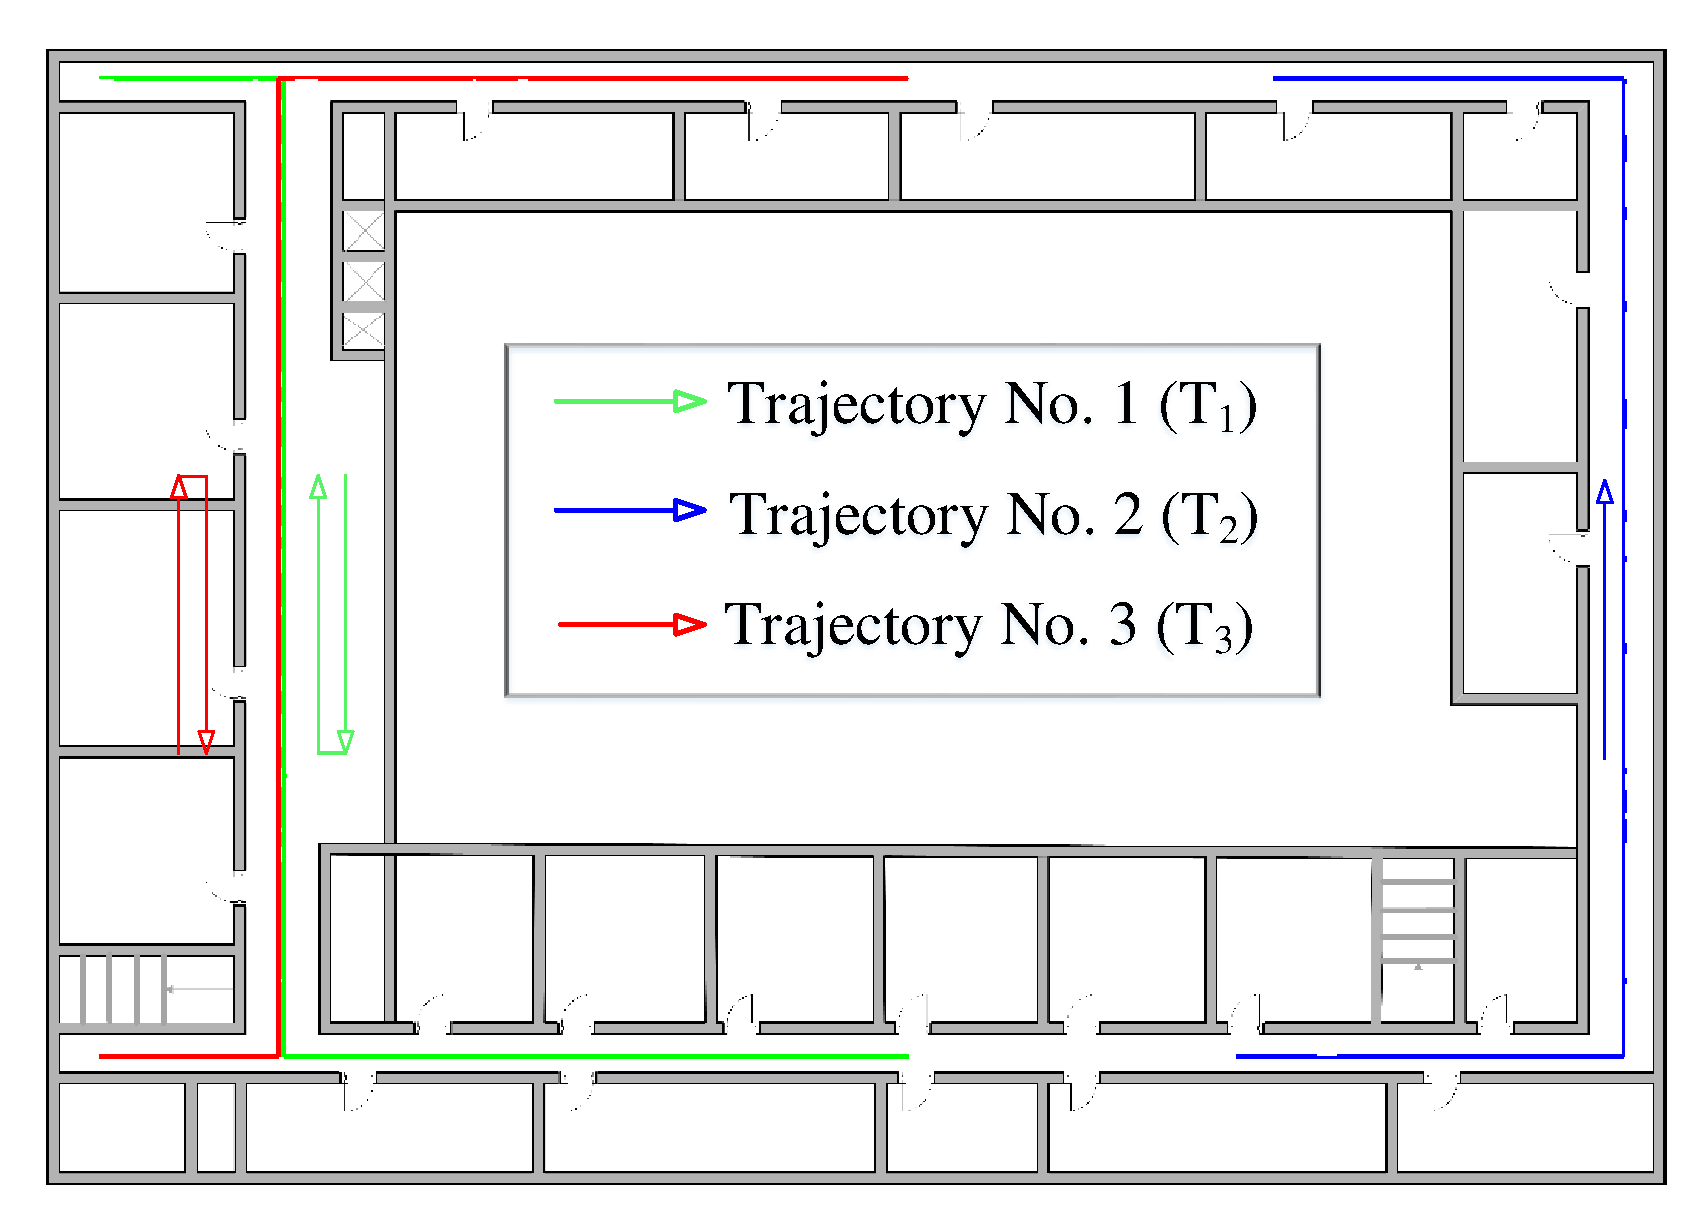
\includegraphics[width=2.325in]{AiFiMatch-Environment}%
		\label{fig-envionment}}
	\hfil
	\subfloat[$T_1\ Offline\ Positioning\ Results$]{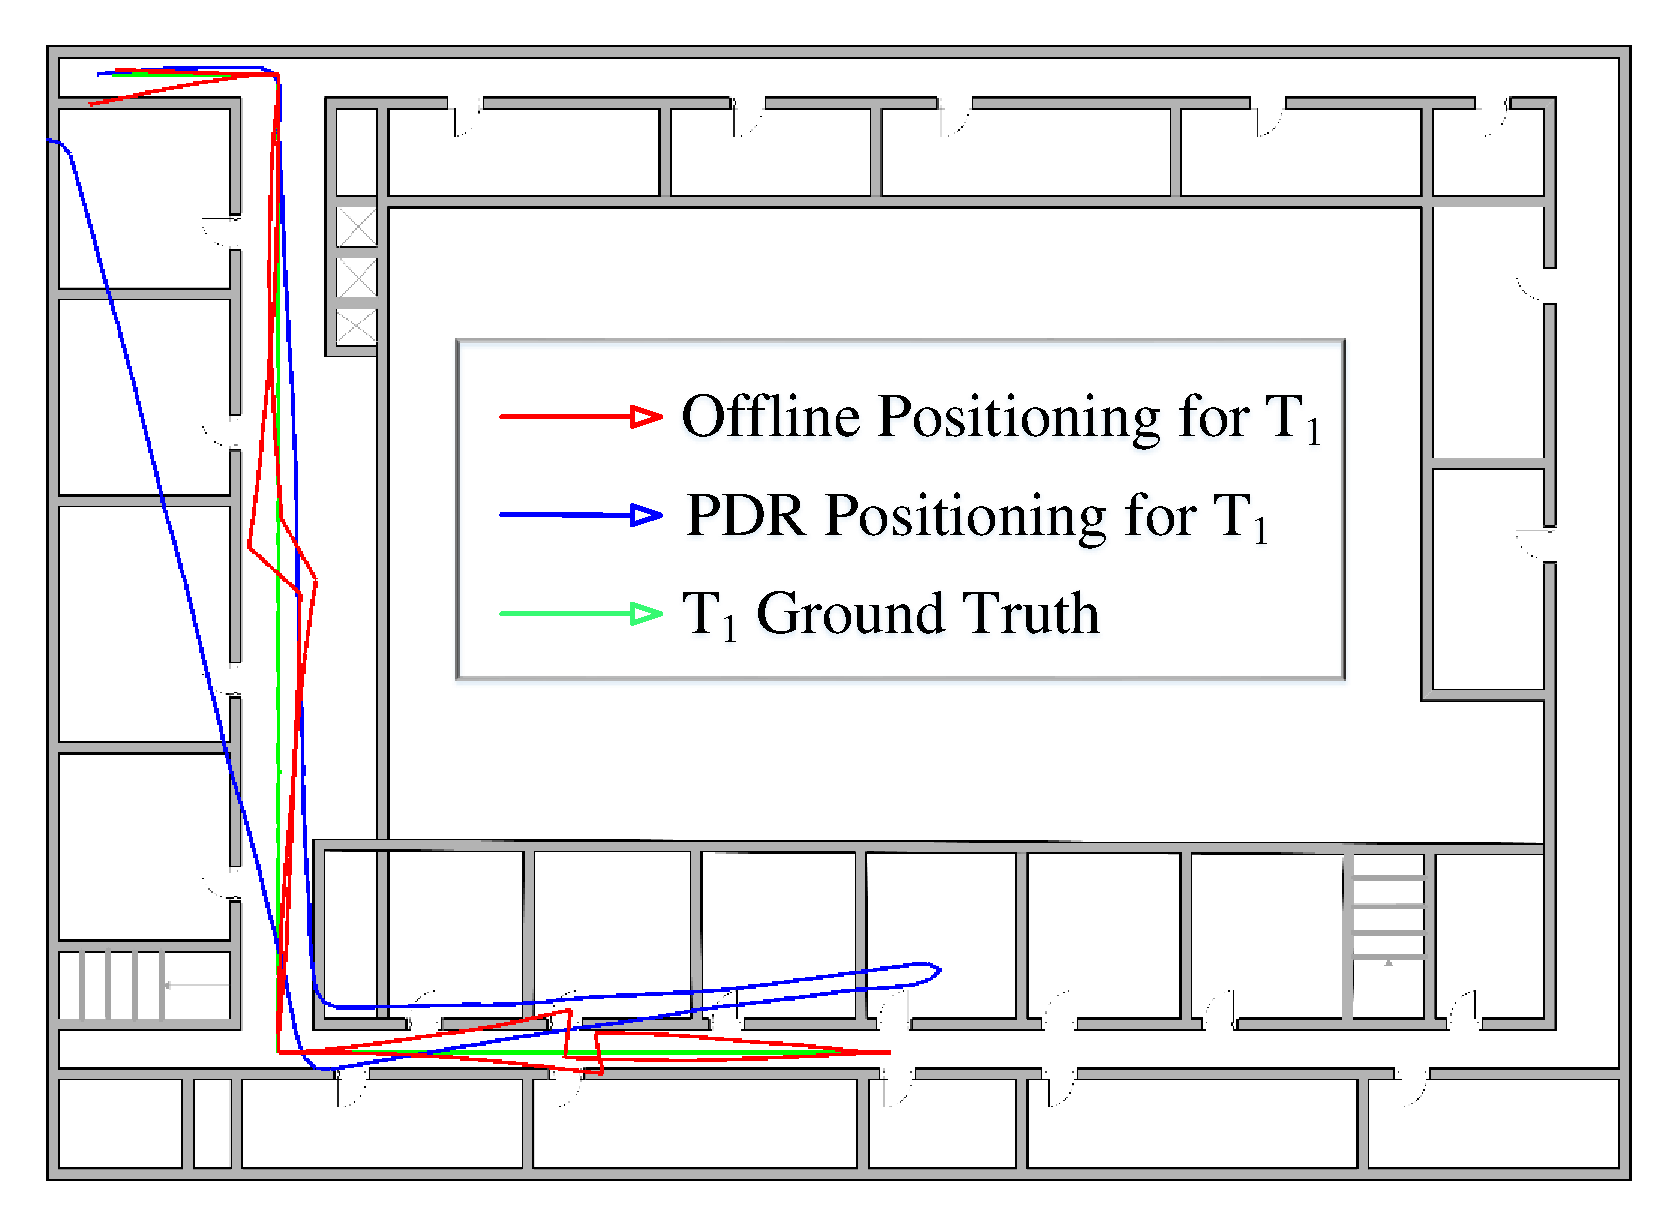
\includegraphics[width=2.282in]{AiFiMatch-OfflineTraject1}%
		\label{fig-offlineT1}}
	\vfil
	\subfloat[$T_2\ Offline\ Positioning\ Results$]{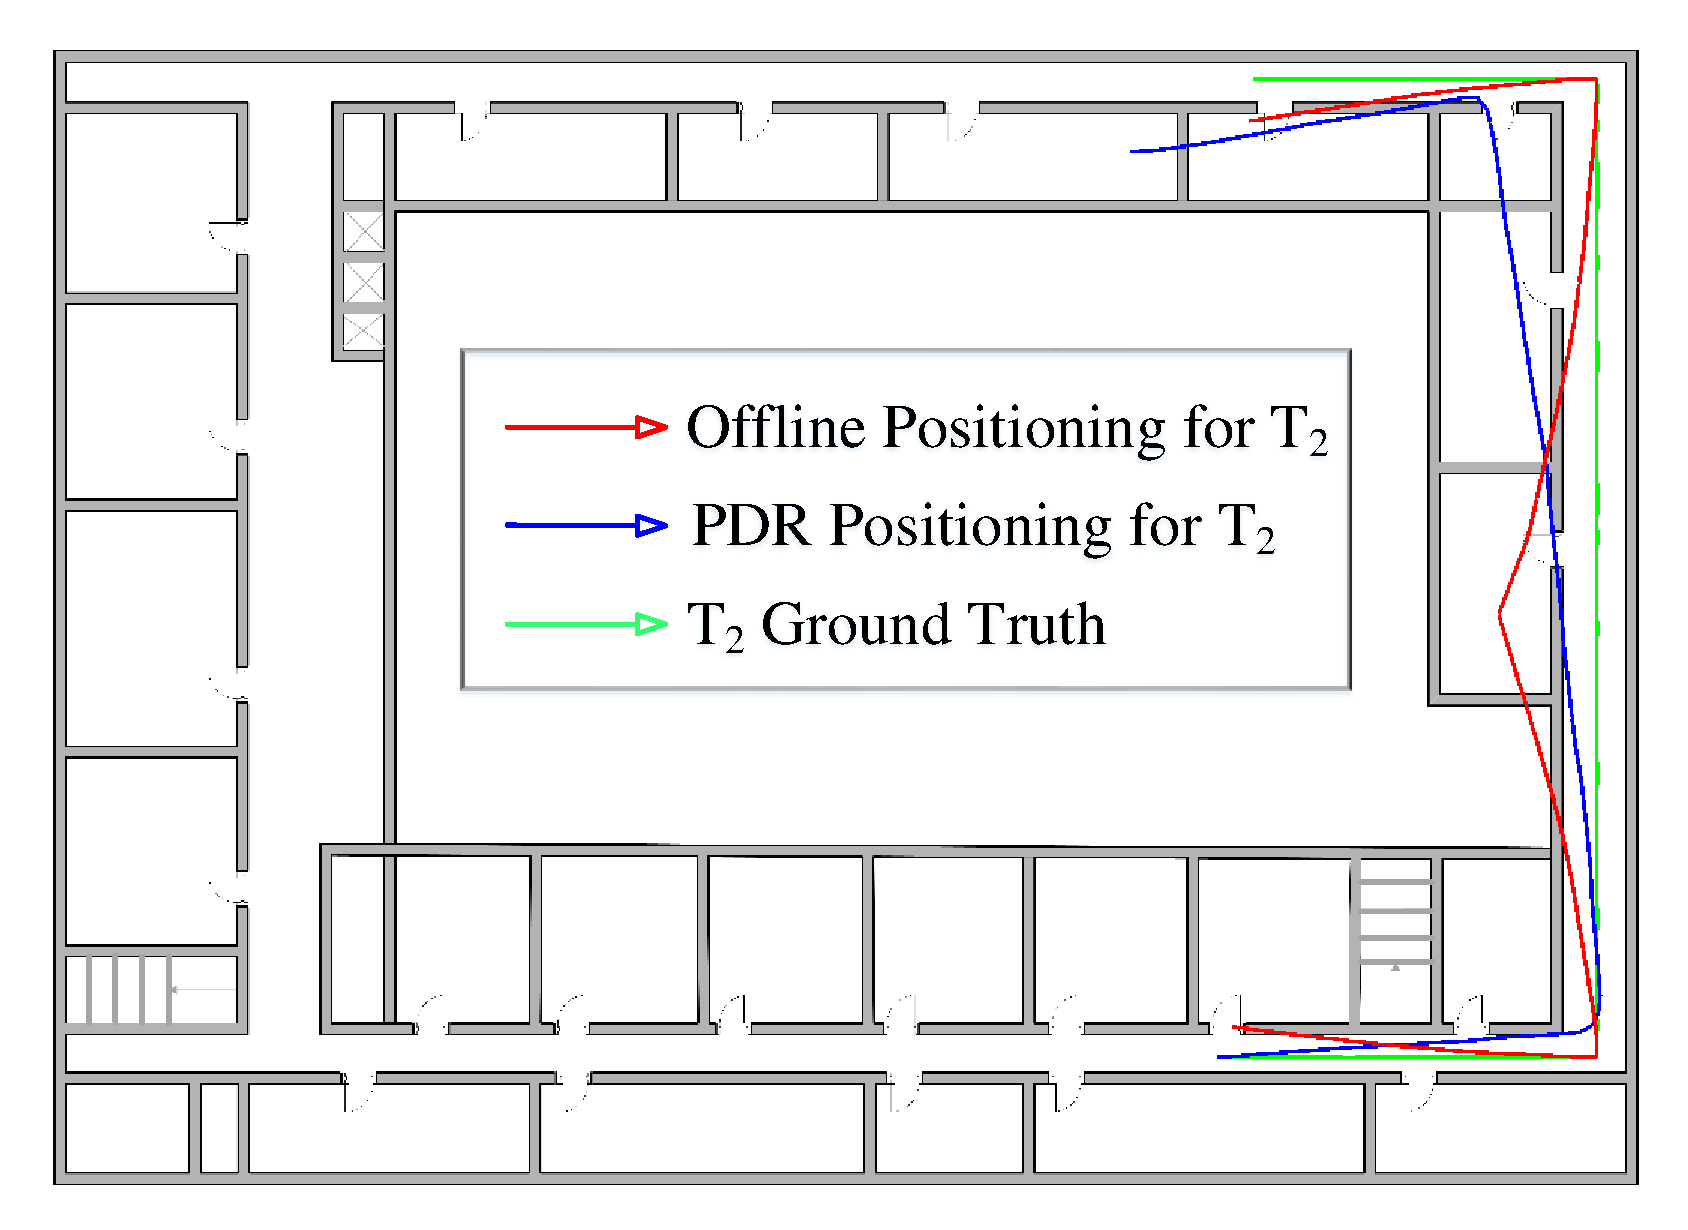
\includegraphics[width=2.3in]{AiFiMatch-OfflineTraject2}%
		\label{fig-offlineT2}}
	\hfil
	\subfloat[$T_3\ Offline\ Positioning\ Results$]{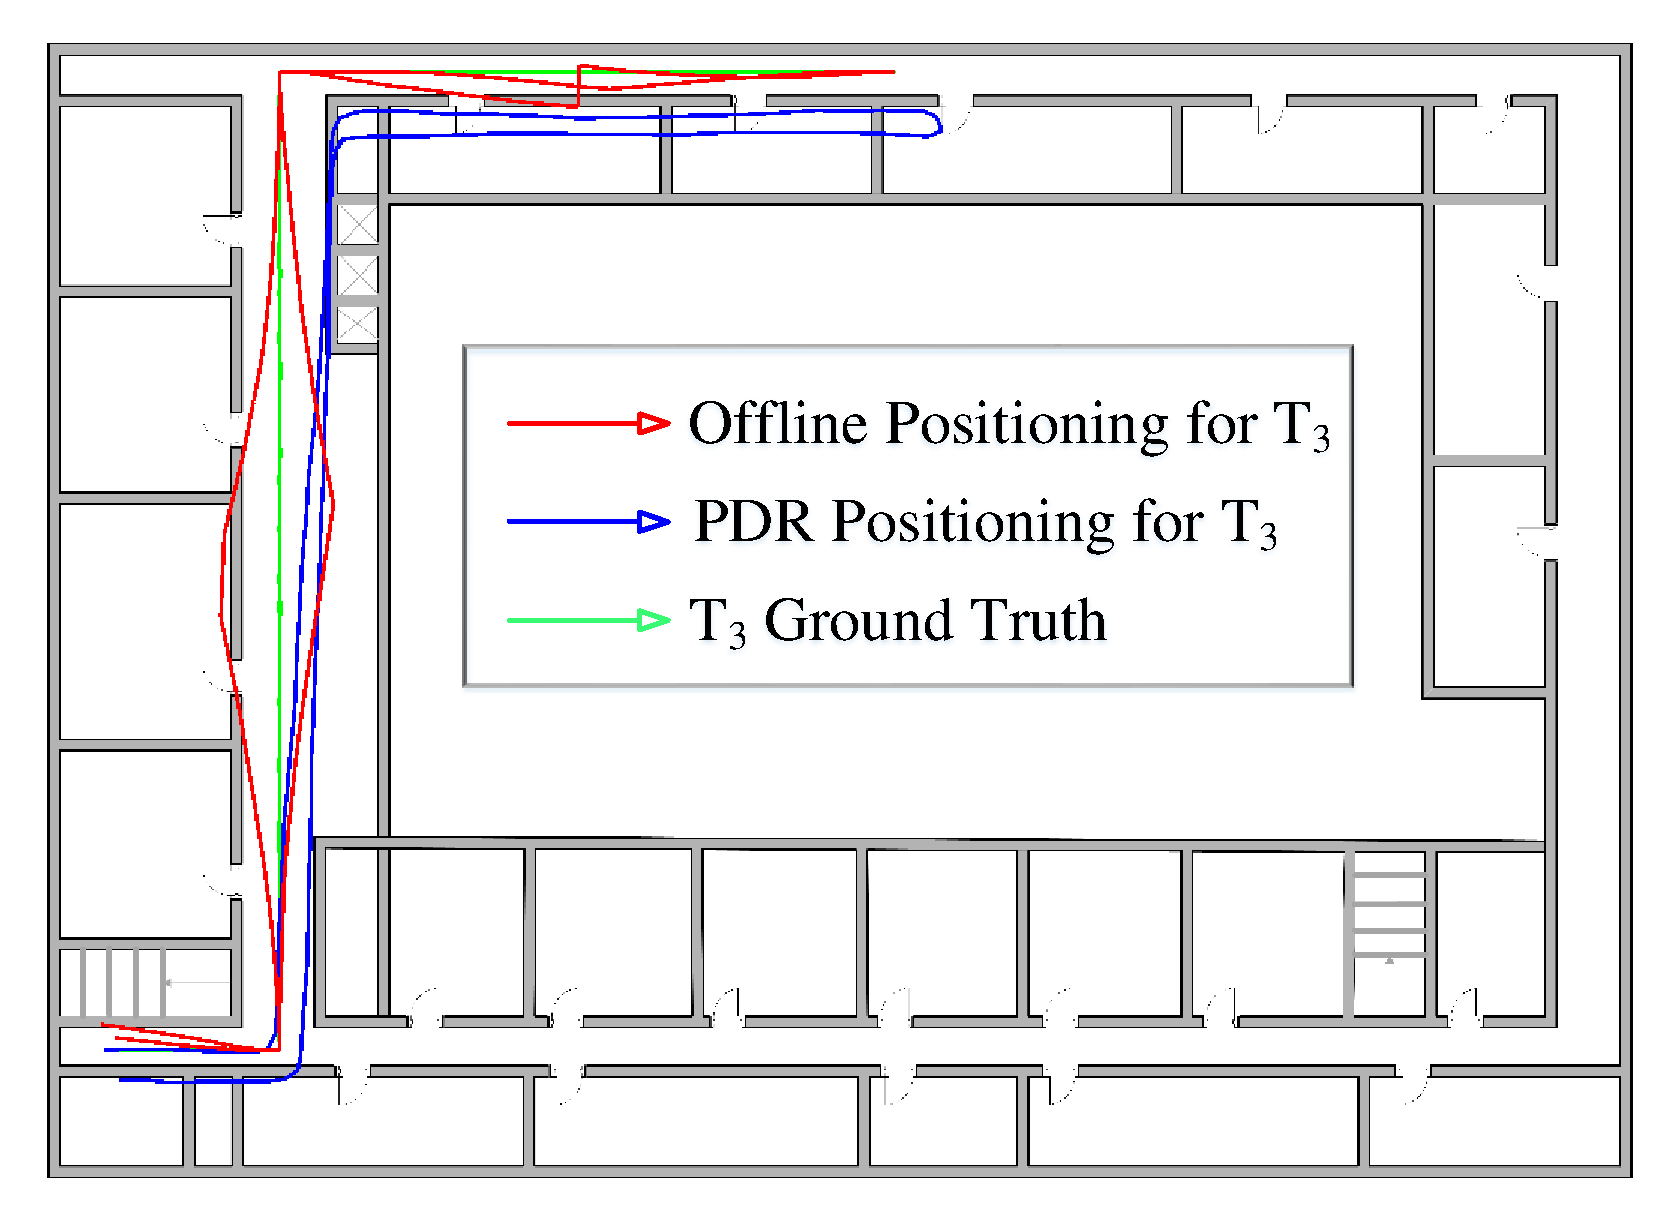
\includegraphics[width=2.3in]{AiFiMatch-OfflineTraject3}%
		\label{fig-offlineT3}}
	\caption{ Environment setup and offline positioning results for each trajectory}
	\label{fig-envandoffline}
\end{figure*}
\vspace{-10pt}


\begin{table}
	\newcommand{\tabincell}[2]{\begin{tabular}{@{}#1@{}}#2\end{tabular}}
	\label{tab-offline}
	\caption{Evaluation Results}
	\begin{center}
		\begin{tabular}{|c | c | c | c | c | c | c |}
			\hline
			 \bfseries \tabincell{c}{Trajectory\\ No.}  & \bfseries Length (m) & \bfseries \tabincell{c}{Mean\\ Error (m)} & \bfseries \tabincell{c}{Step\\ Number} &  \bfseries \tabincell{c}{Detected\\ Step} & \bfseries \tabincell{c}{Activity\\ Number} & \bfseries \tabincell{c}{Detected\\ Activity} \\
			\hline
			\bfseries 1 & 176.1 & 1.09 & 238 & \bfseries 240 & 5 & 5 \\
			\hline
			\bfseries 2 & 84.6 & 1.65 & 114 & 114 & 3 & 3  \\
			\hline
			\bfseries 3 & 175.9 & 1.19 & 228 & \bfseries 227 & 5 & 5  \\
			\hline
		\end{tabular}
	\end{center}
\end{table} 

\section{Conclusion}

This paper proposed AiFiMatch: a novel map matching Algorithm based on activity detection and crowd-sourced Wi-Fi for indoor pedestrian tracking and positioning. AiFiMatch leverages the smartphone's motion sensors to detect different activities using a decision tree and then divides the walking trajectory into trajectory subset sequence. The HMM model is used to match walking trajectory subset sequence to road segments sequence.  AiFiMatch can also construct and update fingerprint database based on road segment by crowd-sourcing. We provided the AiFiMatch's system architecture and presented the details of different modules. The performance of AiFiMatch has been evaluated by experiments in a building on campus. The results show that AiFiMatch can track pedestrian's trajectory accurately even without known initial point and is robust to a certain degree of step length and heading direction errors. In addition, with the help of Wi-Fi fingerprints, AiFiMatch reaches convergence quickly and effectively solves the multiple hypotheses caused by symmetry of building structure. 

%
% ---- Bibliography ----
%
\bibliographystyle{splncs}
%\bibliographystyle{splncs03_unsrt}
%\bibliographystyle{unsrt}
%% ------ update by springer lncs ----- %%
%\bibliographystyle{splncs04}
\bibliography{AiFiMatch}

\end{document}
